%This chapter starts off with details of the requirements analysis for the library of SDR IP blocks. It then goes on to discuss the design process and operational design for the proposed library. Thereafter, it describes both hardware and software tools that will be used in order to pave the way for the best development and testing environment. Then the final section overviews the experimental test for each of the designed IP blocks.
\chapter{\label{ch:methodology} Methodology}

\section{Methodology Outline \label{sec:method-outline}}

Quantum computers offer considerably more powerful computing capabilities in comparison to classical computers. However, challenges in realising qubits with long enough decoherence times make quantum computing platforms make them difficult to implement, and therefore exorbitantly expensive to manufacture and maintain. To circumvent some of the challenges that arise with building physical quantum computers, simulations and emulations of quantum computers that are modelled using classical bits offer more accessible and affordable solutions for testing useful quantum algorithms. In this paper, the design of a FPGA-based quantum computer emulator is proposed. In particular, the design is focused on emulation of the 3-qubit QFT quantum circuit and its application in the quantum factoring algorithm, as well as implementation of Grover's search algorithm in finding the index of an entry in a database with 4 elements. Notably, applications of quantum circuits in quantum algorithms require careful consideration of the quantum gate operations corresponding to unitary matrices that transform qubit state vectors. This requirement is due to the fact that as the number of qubits $n$ increases, computational resources that are necessary for simulating the $2^n \times 2^n$ dense matrices increase exponentially. 

Although CPU and GPU-based quantum computer simulations exists, the intrinsic parallelism and customisability offered by FPGAs can greatly improve the design and implementation of these types of simulations. Furthermore, parallelism of CPU and GPUs is limited by the number of cores which can run different threads in a pool to perform computations, whereas FPGA allow designers to specify combinational logic in hardware to reduce latency while producing the correct output of a quantum algorithm. Programmable logic blocks and wire networks in the FPGA fabric facilitate fine-grained parallelism which can be used to implement properties of qubits such as superposition by performing multiple operations simultaneously. Lastly, CPU and GPU-based simulations may become resource intensive and require a lot of memory and processing power to model quantum gates in a quantum circuit. 

In addition to the emulation of quantum algorithms using the logic blocks of FPGAs as quantum gates, a method for simulating a quantum interface for initialising and transmitting single-photon qubits in quantum communication protocols is developed to model the use of quantum dots for exciton emissions. Simulations of single-photon qubit behaviours that satisfy Divincenzo's criterion are performed on a microcontroller that initialises qubits on the FPGA through a light sensing interface that models exciton emissions due to incident laser pulses on a GaAs quantum dot using LEDs, BJTs and LDRs on a veroboard circuit. 

The no-cloning theorem that prohibits the duplication of quantum states makes quantum computing techniques suitable for performing secure communications. Of interest to this study is the application of quantum interfaces for initialising qubits and performing QKD through a quantum protocol that allows a sender, Alice, to transmit secure data through a quantum channel to a receiver, Bob. In this communication schema, the sender Alice, is represented by the microcontroller, while the receiver Bob, is represented by the FPGA. On the microcontroller, qubits and their operations are modelled using C language, while quantum computer operations are synthesised to hardware using VHDL. 

This chapter provides an overview of the research methodology and the different phases in the design process. The methodology is summarised in an overview diagram, followed by an in-depth description of the FPGA emulator system design and the simulation of the quantum interface using an ARM-based STM32 microcontroller. Sections detailing the research methods employed and the phases of the research project precede the system requirement analysis of the quantum emulator and quantum interface. Following the system analysis, a solution is proposed with a description of the design process and operational design for the quantum emulator. Thereafter, the chapter describes both hardware and software tools that will be used in order to efficiently design and synthesise the quantum simulation in the fabric of the FPGA. In the final section, an overview of the experimental test for each of the subsystems is provided. 

\subsection{Phases in the Research and Design Process \label{subsec:method-phases}}

The four phases of the iterative design and research methodology are illustrated in figure \ref{fig:methodology-phases} below. In the first phase, initial system requirements regarding FPGA simulation of quantum computers and the input and output data that is transmitted in quantum interfaces that facilitate communication through a quantum channel were defined. From the design brief, system requirements included PC-based software that can be used to send and receive data for processing in the emulated quantum computer.    
\begin{figure}[!ht]
	\centering
	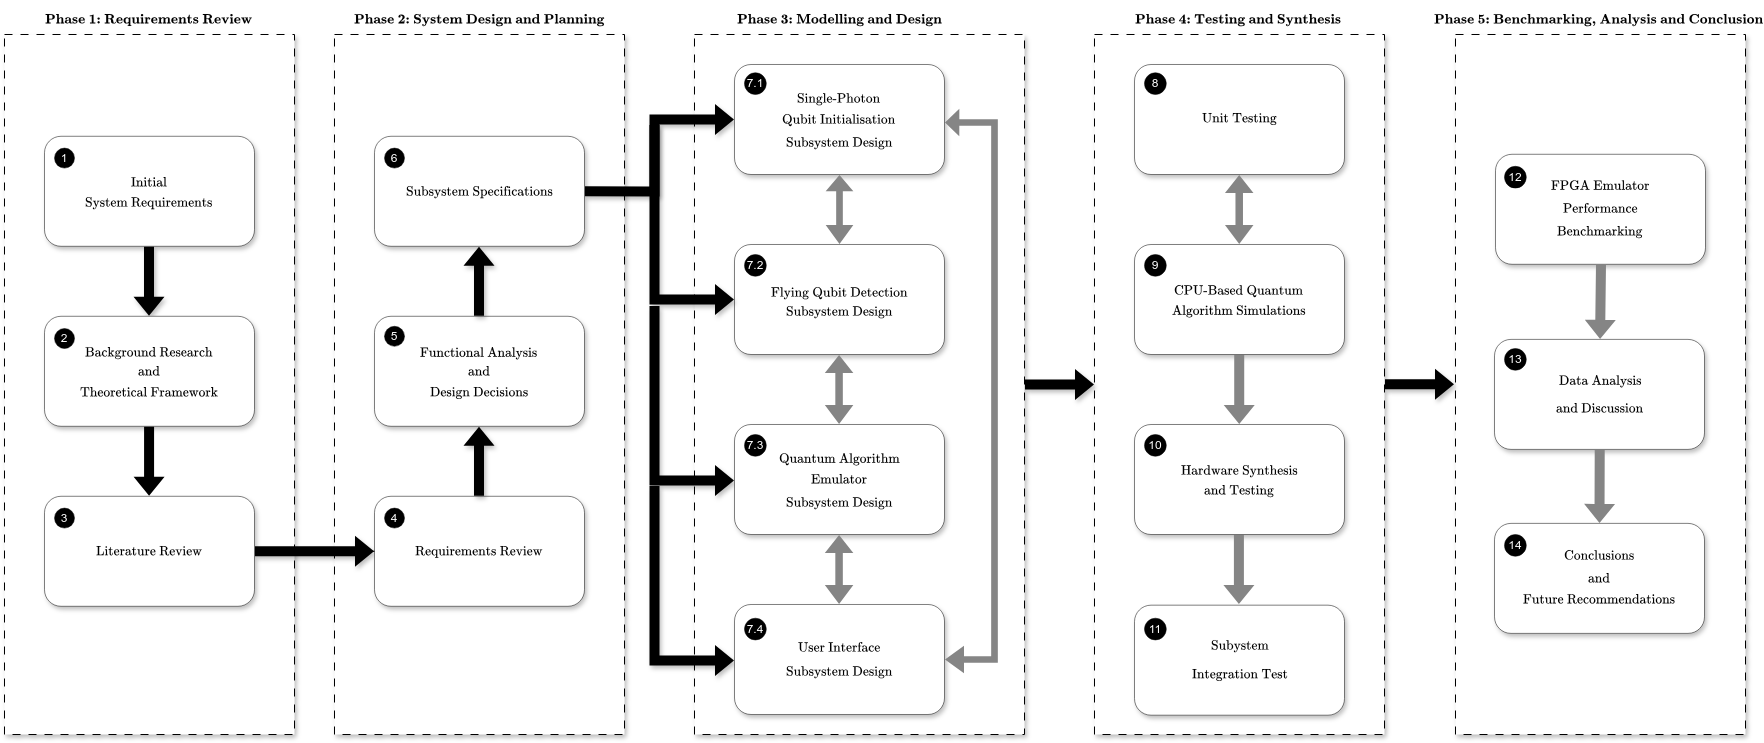
\includegraphics[width=1.0\linewidth]{body/ch4/figs/methodology-phases}
	\caption[Methodology Overview Diagram.]{Methodology overview diagram showing the four phases of the iterative design process, with each step indicated by a block and the direction of flow of critical data between steps presented by the arrows. The flow of data that does not affect the sequence of the development process is represented by the grey arrows.}
	\label{fig:methodology-phases}
\end{figure}
Following the documentation of initial requirements in the first phase, thorough background research was undertaken to formulate a theoretical framework that can reduce the multi-disciplinary concepts in quantum computing to a mathematical description that accurately describes the quantum algorithms involved. This theoretical framework was used to inform the literature review, which goes into details about previous implementations and designs of different quantum computers and their simulations on FPGA as seen in chapter \ref{ch:lit_review}. Summaries of reviewed literature concluded the first phase of the development.

The second phase began with a review of the requirements incorporating the theoretical framework and methodologies proposed in literature. A review of the requirements assisted in making design decisions about the technical subsystems specifications that can fulfil the requirements. In the third phase the quantum computer emulator and quantum interface model design was divided into four subsystems, namely:
\begin{itemize}
	\item 
	Single-Photon Qubit Initialisation Subsystem (SPQIS)
	\item
	Flying Qubit Detection Subsystem (FQDS)
	\item 
	Quantum Algorithm Emulator Subsystem (QAES)
	\item 
	User Interface Subsystem (UIS)
\end{itemize}
The Single-Photon Qubit Initialisation subsystem electronically models the preparation pulses of weak coherent qubit states using a monochromatic laser. This subsystem interacts with the FLying Qubit Detection Subsystem which encapsulates the model of a quantum dot single-photon detector that prepares the quantum states for emulation on the FPGA using appropriate quantum gates at the input. The emulation of quantum gate operations on the detected quantum states is specified in the Quantum Algorithm Emulator subsystem which also performs the quantum factoring and quantum search algorithms using the QFT and oracle subroutines. The modular operation of the quantum emulator was described using VHDL and synthesised for hardware in the Xilinx Vivado development toolkit. Lastly, users can interact with the emulated quantum computer through the electronics model of a quantum channel that is managed by an ARM-based control unit. A C program was used to facilitate the interface between the user and the classical-quantum system.  

A unit test is performed on the system where the functional operation of each subsystem is verified. Results are compared to CPU-based simulations of each model using appropriate software including MATLAB, LTSpice and other CAD tools before the VHDL code is synthesised and tested. The performance of the emulated quantum system is benchmarked using a Python implementation of the algorithm as the golden measure and a quantum computer simulation in MATLAB for further comparison. Finally, a discussion and analysis of the results is presented, before conclusions are drawn and future recommendations are made on the overall design of the system. 

The overall development process follows a variation Waterfall development process which requires sequential completion of each phase before the next one starts and a process checking mechanism with high level design validation by subsystem integration tests.

\section{System Requirements \label{sec:method-sys-requirements}}

System requirements were derived from the project brief detailing the emulation of a quantum computer on a FPGA, and from the concepts explored in existing implementations from literature. This section also details the requirements for the implementation of a quantum interface that can transmit data between a classical and quantum computer. Additional design requirements were introduced according to the constraints that are imposed on a quantum computer by the behaviour and quantum mechanical properties of qubits. Ultimately, the initial system requirements occasioned were divided into user, functional and non-functional requirements.

\subsection{User Requirements \label{subsec:method-user-req}}

The following user requirements were extracted from the project brief.

\begin{table}[ht!]
	\centering
	\caption[User System Requirements.]{Showing the user requirements for the FPGA-based quantum computer emulator system.}
	\label{tab:urs}
	\begin{tabular}{ |c|c| } 
		\hline
		\textbf{Label} & \textbf{Name}\\ 
		\hline
		UR01 & Simulation of Quantum Computer \\ 
		\hline
		UR02 & Interface for Quantum Computing \\ 
		\hline
		UR03 & Execution of Quantum Algorithms \\ 
		\hline
		UR04 & Real-Time Results Display \\ 
		\hline
	\end{tabular}
\end{table}

The following gives a short description of the user requirements as listed in the table above:
\begin{itemize}
	\item 
	\textbf{UR01} - The system must be capable of simulating the behaviour of a quantum computer on a FPGA, representing qubits and quantum operations like Grover's algorithm and the QFT. 
	\item 
	\textbf{UR02} -  The system requires a PC-based interface to send and receive data from the FPGA-based quantum simulator. This includes a GUI for entering inputs and visualising the output from the quantum programs.
	\item 
	\textbf{UR03} - The system should allow users to execute trial quantum programs like Grover's algorithm and the QFT, or other simple algorithms such as key matching or code cracking.
	\item 
	\textbf{UR04} - Users need real-time visualisation of quantum simulation results and the output data structures involved in the quantum experiments performed. 
\end{itemize}
\subsection{Functional Requirements \label{subsec:method-functional-req}}

Table \ref{tab:frs} details further requirements derived from insights gained through research.
\begin{table}[ht!]
	\centering
	\caption[Functional System Requirements.]{Showing the functional requirements for operation of the FPGA-based quantum computer emulator system.}
	\label{tab:frs}
	\begin{tabular}{ | c | c | } 
		\hline
		\textbf{Label} & \textbf{Name} \\ 
		\hline
		FR01 & Qubit Simulation \\ 
		\hline
		FR02 & Quantum Algorithm Emulations \\ 
		\hline
		FR03 & FPGA and PC Interface \\ 
		\hline
		FR04 & Graphical User Interface \\ 
		\hline
		FR05 & Data Transfer and Processing \\ 
		\hline
		FR06 & Correctness and Emulation Accuracy \\ 
		\hline
		FR07 & Error Handling \\ 
		\hline
	\end{tabular}
\end{table}

Corresponding descriptions of the functional requirements are listed below:
\begin{itemize}
	\item
	\textbf{FR01} - The system must simulate the behaviour of qubits according to DiVincenzo's five criteria for the realisation of quantum computers.
	\item
	\textbf{FR02} - The system must implement and run quantum circuits for performing the quantum search algorithm, and for the application of the QFT in performing useful operations using a quantum computer. 
	\item 
	\textbf{FR03} - The system must facilitate seamless communication between the FPGA quantum emulator and another classical device. The software should send input data to the FPGA, trigger the quantum computation and receive the results for display in the GUI.
	\item 
	\textbf{FR04} - The GUI must include a PC-based GUI that allows users to input required parameters for quantum computations and display the output from the quantum computations in a user-friendly manner.
	\item 
	\textbf{FR05} - Data transfer must be facilitated efficiently, ensuring that the communication delays are minimised while maintaining a moderate to high data accuracy. 
	\item 
	\textbf{FR06} - The FPGA quantum emulator should implement algorithms to produce accurate and expected results.
	\item 
	\textbf{FR07} - The system must identify and report errors such as inputs that cannot be processed by the quantum computer or failures in the system.
\end{itemize}

\subsection{Non-Functional Requirements \label{subsec:method-non-funct-req}}

The non-functional requirements listed below define the quality characteristics and operational constraints of the system as shown in table \ref{tab:nfrs}.
\begin{table}[ht!]
	\centering
	\caption[Non-Functional System Requirements.]{Showing the non-functional requirements for operation of the FPGA-based quantum computer emulator system.}
	\label{tab:nfrs}
	\begin{tabular}{ | c| c | } 
		\hline
		\textbf{Label} & \textbf{Name} \\ 
		\hline
		NFR01 & Performance \\ 
		\hline
		NFR02 & Scalability  \\ 
		\hline
		NFR03 & Usability and Portability\\ 
		\hline
		NFR04 & Resource Efficiency\\ 
		\hline
	\end{tabular}
\end{table}

Descriptions of the non-functional requirements are listed below:
\begin{itemize}
	\item 
	\textbf{NFR01} - The FPGA emulator must simulate qubits, quantum circuits and quantum gates with suitable execution times, although the times may will not match the speed of a real quantum computer.
	\item 
	\textbf{NFR02} - The emulator and quantum interface should be designed modularly in order to support the simulation of quantum computers with more qubits for performing other quantum algorithms in the future.
	\item 
	\textbf{NFR03} - The GUI must be easy to navigate while showing all the necessary information that can also help users who are unfamiliar with quantum computing concepts. The software should run on commonly used operating systems such as Windows or Linux.
	\item 
	\textbf{NFR04} - Resource usage, memory and computational overhead must be minimised to optimise FPGA capabilities and speedup execution times.
\end{itemize}

These requirements were used guide the development of the FPGA-based quantum emulator while adhering to the mathematical and physical constraints that stipulate the existence of quantum computers. 

\section{Requirements Analysis \label{sec:method-req-analysis}}

Emulation of quantum computers is a challenging task due to the fundamental differences between qubits and classical bits and the dense matrix operations involved in quantum circuits. While classical bits, are commonly produced by alternating voltage levels between a high and low value, qubits can be realised using different particles in quantum systems such as atoms, electronics and photons. Thus, prudent analysis of the type of quantum computer that is modelled in the design was necessary for accurate simulations. This section provides an expansion of the user, functional and non-functional requirement based on accrued theoretical and research background knowledge of quantum computing. 

\subsection{Description of Design Modularisation}

To fulfil the requirements, the proposed system was modularised into the four subsystems listed above. Figure \ref{fig:overall-system-architecture} illustrates an overview of the subsystems and their interactions.
\begin{figure}[!ht]
	\centering
	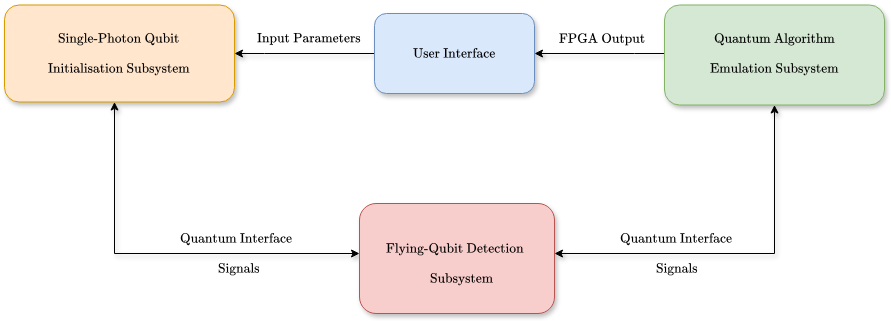
\includegraphics[width=\linewidth]{body/ch4/figs/overall-system-architecture}
	\caption[Subsystem Block Diagram.]{Overview system diagram showing the flow of data and instructions. A quantum computer is emulated on the FPGA belonging to the Quantum Algorithm Emulation subsystem.}
	\label{fig:overall-system-architecture}
\end{figure}

The figure also illustrates the proposed devices in the system, including an ARM-based microcontroller, FPGA, an electronic circuit for modelling the quantum interface, and a PC as part of the SPQIS and UIS modules. To compensate for differing operating frequencies, the proposed solution does not use a clock to synchronise the blocks. Instead, subsystems can communicate through \texttt{trigger} and \texttt{enable} signals to indicate the \texttt{start} and \texttt{end} of a process.

\subsubsection{Single-Photon Initialisation Subsystem}
The SPQIS initialises well-characterised qubits and defines the decoherence times of each qubit. To achieve this, the subsystem generates the probabilities of the quantum states of each qubit and interacts with the UIS to allow users to define the parameters that characterise the simulated quantum computer. Optimisation of the SPQIS involves considerations of accurate qubit representations, memory usage, and suitable preparation of qubits for transmission through the quantum channel in the FQDS. In turn, the manner in which qubits are prepared has an effect on the transmission rate of the quantum channel which can be measured as the number of flying qubits that are transmitted per second. The SPQIS is mainly facilitated on an ARM-based microcontroller. On the FPGA, the SPQIS manages the parameters of detected qubits through the circuit modelling the quantum channel. As shown in figure \ref{fig:overall-system-architecture} SPQIS is composed of:
\begin{itemize}
	\item 
	A pseudo-number generator for satisfying the initialisation of well-characterised, fiducial qubit quantum state	
	\item 
	Data structures and memory for storing qubit parameters
	\item 
	ARM-based microcontroller for initialising qubit
	\item 
	FPGA-based quantum computer emulator for initialising qubits as inputs to the quantum circuit or quantum algorithm performed
	\item 
	Electronic circuit that models flying qubits at the output
\end{itemize}
An overview of the SPQIS is illustrated in figure \ref{fig:spqis-overview} where a user prepares 3 physical qubit modelled in the quantum channel electronic circuit. Physical qubits are propagated through the quantum channel and detected by sensors in the FQDS module facilitated by the FPGA quantum computer emulator. 
\begin{figure}[!ht]
	\centering
	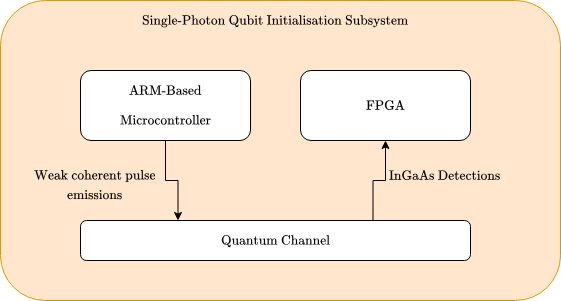
\includegraphics[width=\linewidth]{body/ch4/figs/spqis-overview}
	\caption[Single-Photon Qubit Initialisation Subsystem (SPQIS) Overview.]{The proposed design models the initialisation and transmission of single-photon qubits. Qubits are initialised on the microcontroller and mapped to physical qubits which are transmitted through the quantum channel. These "flying qubits" are decoded by the FPGA subsystem.}
	\label{fig:spqis-overview}
\end{figure}

The performance of this subsystem can be assessed from the  transmission rate and the power consumption. 

\subsubsection{Flying Qubit Detection Subsystem}

The aim of this module to model the detection of physical qubits through a quantum channel facilitated by a quantum network in which lasers are used to initialise and manipulate qubits. The main component in the subsystem is the electronic circuit that performs the quantum communication protocols for transmitting qubits between classical systems and a quantum computer. As noted in the literature, the apparatus of a quantum interface must have the ability to inter-convert stationary and flying qubits. Furthermore, the quantum interface should have the ability to transmit flying qubits between the sender's and receiver's private spaces \cite{divincenzo2000physical}. 

To fulfil this requirement, the proposed solution models photodetectors that convert flying qubits into stationary qubits. Flying qubits are propagated through the quantum channel modelling a fibre optic cable as illustrated in \ref{fig:fqds-overview}. 
\begin{figure}[!ht]
	\centering
	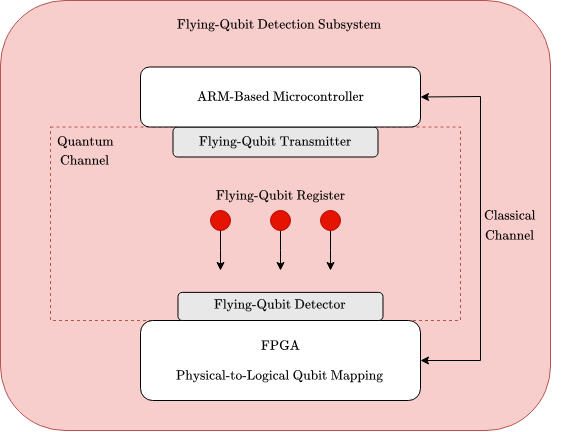
\includegraphics[width=0.85\linewidth]{body/ch4/figs/fqds-overview}
	\caption[Flying-Qubit Detection (FQDS) Subsystem Overview.]{Physical qubits are transmitted through the quantum channel in the FQDS module which enables physical qubits to be mapped to logical qubits on the FPGA system. The flying-qubit transmitter (CW laser) is modelled using LEDs, while the flying-qubit detector is modelled in a series of photoresistors or LDRs.}
	\label{fig:fqds-overview}
\end{figure}

The output from the photodetectors is transferred to the FPGA which encodes the physical qubits to logical qubits that can be used to perform quantum algorithms. The FQDS system consists of:
\begin{itemize}
	\item 
	A model of a fibre link that provides a secure path for the propagation of flying qubits
	\item 
	Electronic circuit with photodetectors for converting flying qubits to stationary physical qubits
	\item 
	FPGA for mapping physical qubits to logical qubits
\end{itemize}
The proposed solution models a bit-mapping gate by using the photodetectors to capture flying qubits in intervals, or detection windows. The number of qubits detected by the sensors needs to match the number of qubits transmitted from the SPQIS. Therefore, the performance of the FQDS is characterised by the decoherence times of the flying qubits, as well as the qubit detection rate. Consequently, the ratio between the qubit transmission rate and qubit detection rate is used to define the efficiency of the quantum channel. 

\subsubsection{Quantum Algorithm Emulator Subsystem}

To successfully implement quantum algorithms, the QAES defines a universal set of quantum gates and quantum circuits that describe the sequence operations on the qubits at the output of the FQDS. Since the QAES system is FPGA based, a high-level design and verification development workflow is proposed. Then, quantum gate operations are mapped to FPGA logic. Thereafter, the system is verified using RTL simulations before synthesising each block. Since quantum gate operations require manipulation of dense matrices which can lead to storage overheads, the memory schemes proposed aim exploit the capabilities of the FPGA by using a combination of distributed RAM and FIFO shift registers for storing quantum state information. The QAES system components include:
\begin{itemize}
	\item 
	A set of universal quantum gates
	\item 
	Quantum circuits for executing quantum algorithms
	\item 
	HDL code for synthesising quantum algorithms to the system architecture
	\item 
	FPGA hardware for emulating a quantum computer with onboard logic cells, DSP blocks and various IP cores
	\item 
	External memory for storing quantum state information and extending the storage capabilities of the FPGA	
\end{itemize}
The QAES system takes the output of the FQDS module and performs a quantum algorithm based on the user parameters defined in the SPQIS through the UIS module. The subsystem communicates with the ARM-based microcontroller to synchronise communication through the quantum channel. The output of the emulated quantum computer is a classical binary code that is returned to the UIS at the end of an algorithm. The UIS also allows users to select the quantum circuit or quantum algorithm to be performed by the QAES on the FPGA. 

Figure \ref{fig:fpga-design-flow} illustrates the design flow of the FPGA. The process begins with creating the register-transfer level (RTL) to match the functionality of the quantum algorithm to the hardware logic while operating on a data stream of qubits. 
\begin{figure}[!ht]
	\centering
	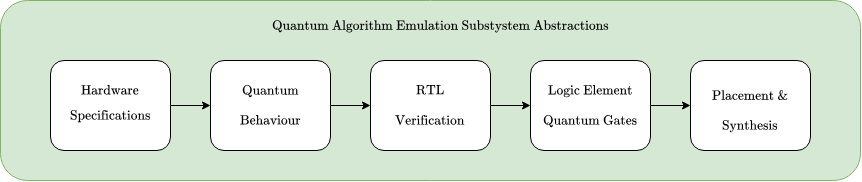
\includegraphics[width=1.0\linewidth]{body/ch4/figs/fpga-design-flow}
	\caption[Design Abstraction of FPGA-Based Quantum Computer Emulator.]{Due to the limited information in the system requirements, a top-down approach is adopted in order to add function details to the FPGA quantum emulator.}
	\label{fig:fpga-design-flow}
\end{figure}

The verification step ensures that the design works for the intended hardware architecture through appropriate testbench implementations. In the synthesis step, software development tools are used to transform RTL code representing quantum gate operations to digital logic gates and attempts to meet the register-to-register clock frequency while minimising resource usage on the FPGA. The FPGA system is integrated to the overall system, followed by implementation which produces a bitstream that is loaded to the device for FPGA programming. Finally, the QAES is lab tested and debugged using test inputs.

The performance of the FPGA when executing quantum algorithms is compared to the performance of PC-based quantum computer simulators. Furthermore, resource usage is compared to previous implementations of emulated quantum computers on FPGAs. Since power consumption depends on the register-to-register clock frequency and resource usage, the aim of the design is to minimise power consumption by reducing the number of resources required while performing quantum algorithms quickly.

\subsubsection{User Interface Subsystem}

Outputs from the FPGA-based QAES module are displayed graphically using PC-based software and a 7-segment display. The primary objective of the UIS module is to allow users to calibrate the system to run the desired algorithm on the system. Given that quantum algorithms require different qubit preparation techniques and quantum gates, the system also needs to allow users to define the inputs and select the quantum circuit that is required for experimentations. In summary, the UIS module allows users to:
\begin{itemize}
	\item 
	Define the initial qubit states
	\item 
	Select and configure the quantum circuit
	\item 
	Visualise outputs to help users understand the results from the quantum computer
\end{itemize}
The UIS interacts with the SPQIS to allow users to modify qubit preparation parameters before transmission through the quantum channel. Lastly, this subsystem allows users to upload results from the random number generator to the QAES system on the FPGA. 

\subsection{FPGA Resources for Modelling Quantum States \label{subsec:req-sim-qubits}}

For a quantum computer to exist, the qubits in the system need to satisfy the five criterion proposed by DiVincenzo \cite{divincenzo2000physical}. The method used to model qubits directly affects all the  system requirements. The first criterion that the simulated qubits must satisfy in order to accurately model the operation of quantum computing systems is that each quantum state needs to be well-characterised. As noted in the theoretical framework, the polarisation state, $\ket{\psi}$, of a photon, can be represented as a linear combination of the state vectors $\ket{\uparrow}$ and $\ket{\rightarrow}$, with coefficients $\alpha$ and $\beta$ that satisfy the normalisation condition in equation \ref{eqn:normalisation-condition}. Alternatively, qubits can represent the spin-state of atoms and fermions such as electrons. The polarisation states or electron spin-states are mapped to the computational basis set ${\ket{0}, \ket{1}}$. Therefore, in the computational basis, simulated qubit $\ket{\psi}$ should satisfy
\begin{align}\label{eqn:qstate-comp-basis}
	\ket{\psi}	& = \alpha_0\ket{0} + \alpha_1\ket{1}\nonumber\\
	\ket{0} = \left(\begin{matrix}
		1 \\ 0
	\end{matrix}\right)&~~;~~\ket{1} = \left(\begin{matrix}
	0 \\ 1
\end{matrix}\right)\nonumber\\
\ket{\psi} & = \left(\begin{matrix}
	\alpha_0\\
	\alpha_1
\end{matrix}\right)
\end{align}
where the coefficients $\alpha$ represent the wave amplitudes of the quantum state $\ket{\psi}$ that adhere to the normalisation condition derived from the Born postulate of quantum mechanics requiring that
\begin{align}
	|\alpha_0|^2 + |\alpha_1|^2 = 1\nonumber
\end{align}
Since classical bits cannot directly simulate the superposition of quantum states, the above representation of qubits requires more than one bit to store values of the amplitudes and vectors on a classical computer. Therefore, simulating a quantum computer requires the magnitudes of the basis states to be stored in order to model a well-characterised qubit. 

For this design, it can be assumed that if the system has $n$ qubits, then it can represent integer decimal numbers from 0 to $2^n-1$ which can be encoded in the computational basis as a string of bits to represent a multi-qubit state. For instance, a 4-qubit quantum computer is able to represent integers from 0 to 15, whereas a $3$-qubit quantum computer can represent integers from 0 to 7. Therefore, the performance, power consumption and memory usage of the system was expected to increase as the number of qubits $n$ increased. 

In general, the array structure of FPGAs consists of slices which comprise one or more programmable logic blocks; a routing network for interconnecting logic resources; I/O logic to communicate with the outside world; clock managers and hard-macros. The QAES exploits the structure of a FPGA to store and manipulate classical bits that represent quantum information. The methodology explores the application of Xilinx 7-series FPGA architecture in emulating quantum systems. In particular, LUTs and flip-flops can be used for memory as well as sequential and combinatorial logic. The proposed design aims to implement the $n$-input LUTs as both an asynchronous ROM and for performing $n$-input logic functions for quantum gate operations. Figure \ref{fig:amd-lut6} depicts the LUT6s which have 6-bit addressing to construct a 64-bit ROM \cite{amd2024support}. If a LUT6 is used to construct linear mappings between classical bits and the computational basis states, a single table can represent quantum registers with values from $\ket{0}_{10}$ up to $\ket{63}_{10}$ as seen illustrated in the figure. 
\begin{figure}[!ht]
	\centering
	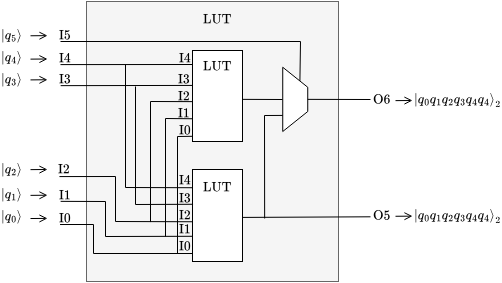
\includegraphics[width=0.85\linewidth]{body/ch4/figs/amd-lut6}
	\caption[Direct Mapping of Computational Basis States to Xilinx FPGA LUTs.]{Illustrating the proposed application of Xilinx 7-series LUTs for directly representing quantum registers for values between $\ket{0}_{10}$ and $\ket{63}_{10}$. The MSB corresponding to I0 is mapped to the qubit $\ket{q_0}$. Similarly, the LSB I5 is mapped to the qubit $\ket{q_5}$ in the quantum register. The output of the LUT represents the pure quantum register with a probability of 1.}
	\label{fig:amd-lut6}
\end{figure}

Each qubit in the quantum register representing a decimal number is associated with an \texttt{INIT} attribute of the FPGA LUT primitive consisting of a 64-bit hexadecimal value. Similar to real qubits, LUTs are initialised to a default value of zero, which implies that at if the inputs of a LUT6 are not specified, then the corresponding initial quantum state register is $\ket{000000}_2$. The  In other words, quantum states are generated from the binary encoding of some integer $\psi_{2}$ as a bit string $(q_0 q_1 \cdots q_{n-1})_2$. For example, when emulating a $6$-qubit quantum register using 6-input LUTs, the integers $\psi_1 = 3_{10}$ and $\psi_2 = 5_{10}$ can be represented in the computational basis as 
\begin{align}
	\ket{\psi}_{2}	& = \ket{q_0 q_1 q_2 \cdots q_{n-1}}_2\nonumber\\
\implies~~	\ket{\psi_1} = \ket{3}_{10} & = \ket{000011}_2 \nonumber\\
	\ket{\psi_2} = \ket{5}_{10}	& = \ket{000101}_2\nonumber
\end{align} 
As noted in the theoretical section, such a multi-qubit system combines the Hilbert spaces of each quantum state as the tensor product
\begin{align}
	\ket{000011}_2	& = \ket{0}\otimes\ket{0}\otimes\ket{0}\otimes\ket{0}\otimes\ket{1}\otimes\ket{1}\nonumber\\
				& = \left(\begin{matrix}
					1\\
					0
				\end{matrix}\right)\otimes\left(\begin{matrix}
				1\\
				0
			\end{matrix}\right)\otimes\cdots\otimes
			\left(\begin{matrix}
				0\\1
			\end{matrix}\right)\otimes
		\left(\begin{matrix}
			0\\1
		\end{matrix}
		\right)\nonumber\\
		& = (0,0,0,1,0,0, ..., 0)^T\nonumber
\end{align}
For the integer $5_{10}$, the equivalent 6-qubit quantum register can be represented as the column vector given by
\begin{align}
	\ket{000101}_2	& = (0,0,0,0,0,1,...,0)^T\nonumber
\end{align}
These examples illustrates that the position of 1 in the column vector corresponds to the value of the number in the computational basis, i.e. when the integer number is $d$, then the position of 1 in the column vector is $d + 1$. This example also illustrates that in the computational basis, to simulate a relatively small integer in a 6-qubit quantum system could require substantial power, memory and resources, such as LUTs and DSP slices. The size of these column vectors grows exponentially with the number $n$ of qubits, as noted previously. For example, to represent the integer 3 in the computational basis of a 12-qubit quantum computer would require double the amount of memory to store the number. In general, a $n$-qubit produces quantum registers that can be represented as a column vector with $2^n$ entries. This has a direct effect on the fulfilment of system requirement NRF04 which states that resource usage, memory and computational overhead should be minimised. Overall, number of LUTs used in the hardware was expected to increase with the number of qubits in system.

\subsection{Emulation Accuracy in Relation to Quantum State Amplitudes}

In addition to the considerations made on the increase in memory and resource requirements as the number of qubits is increased, an inspection of the amplitude coefficients is critical in design the quantum computer emulator. As noted in equation \ref{eqn:multiple-qubit-state}, a 3-qubit wide quantum register representing an integer $\psi$ is in a state of superposition given by
\begin{align}
	\ket{\psi} & = \alpha_0 \ket{000}_2  + \alpha_1 \ket{001} + \alpha_2 \ket{010} + \alpha_3 \ket{011}\nonumber\\& + \alpha_4 \ket{100} + \alpha_5 \ket{101} + \alpha_6 \ket{110} + \alpha_7 \ket{111}\nonumber 
\end{align}
where each $\alpha_{i}$ is a complex probability that satisfies
\begin{align}
	\sum_{i=0}^{7}|\alpha_{i}|^{2} =  1\nonumber
\end{align} 
Since each $\alpha_{i}$ is a complex number, entries in the column vector of the quantum register that are equal to 1 would need to be replaced by two values. Furthermore, the normalisation constraint on the $\alpha_{i}$ coefficients implies that the magnitude of these complex coefficients must add up to 1, i.e. $0 \leq \alpha_{i} < 1$. The accuracy of the quantum emulator in appropriately modelling a quantum computer depends on the resolution of the number scheme chosen as well as the hardware platform on which an experiment is performed. 

For a PC-based compiler, the precision of the number depends on the resolution of the floating-point number in the $\texttt{float}$ data type. The $\texttt{double}$ data type can also store the amplitudes of the coefficients as a 64-bit number. However, floating-point data types on microcontrollers tend to produce code which uses a substantial storage space. The code is generally also slow because of the complexity of simulating floating-point operations. If the numbers were to be stored in complex form, each entry in the quantum state column vector that is non-zero would need two numbers to store information about the qubit in memory. Furthermore, the design needs to be able to handle potential overflow conditions due to multiplication or division operations. Therefore, the representation and storage of the complex coefficients directly affects system requirements FR03, FR05, FR06 and NFR04, in relation to the FPGA and PC interface, data transfer and processing, correctness and resource efficiency.

On a FPGA, a floating-point number can exist as a fixed number of significant digits and scaled using an exponent in some fixed base. FPGAs typically support \texttt{half}, \texttt{single}, and \texttt{double} format types for representing floating-point numbers. The floating-point encoding scheme is maintained by the IEEE/ANSI 754-1985 standard where a basic number utilises an 8-bit exponent and a 24-bit mantissa as illustrated in figure \ref{fig:floating-point}. The standard fixed-point scheme can represent an unsigned number between 0.0 and 255.9906375 or a signed number between -128.9906375 and 127.9906375 using two's complement. The proposed design stores probabilities with four significant numbers, for example, an amplitude of $1/\sqrt{8}$ is stored as 0.3536. 

For quantum state probabilities represented as signed numbers, the range of values that can be presented also depends on the encoding scheme that is used in the method. It is noted however, that the decimal or part of the probabilities of the quantum states is always 0 or 1, thus, the emulation accuracy would mostly depend on the number of mantissa or fractional bits used. 
\begin{figure}[!ht]
	\centering
	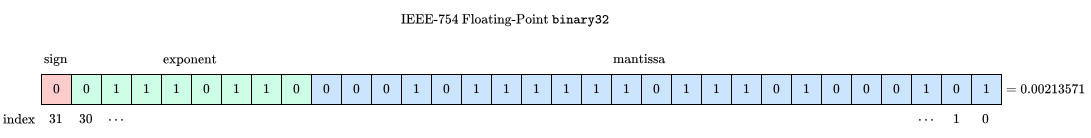
\includegraphics[width=\linewidth]{body/ch4/figs/floating-point}
	\caption[Illustrating the IEEE 754-1985 Standard for 32-bit Floating-Point Numbers.]{The IEEE 754 standard gives precision of 6 to 9 significant decimal digit precision by employing a sign-bit, 8 exponent bits, and 24 mantissa bits with 23 bits that are stored explicitly.}
	\label{fig:floating-point}
\end{figure}
Alternatively, fixed-point numbers use fixed binary point instead of a floating decimal point with a dynamic location based on the value of the exponent. An implied binary point separates a binary number into $u$ integer bits and $v$ fractional bits as illustrated in figure \ref{fig:fixed-point}.
\begin{figure}[!ht]
	\centering
	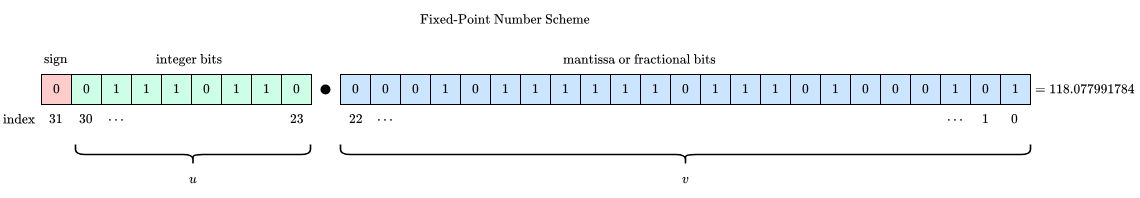
\includegraphics[width=\linewidth]{body/ch4/figs/fixed-point}
	\caption[Illustrating a 32-bit Fixed-Point Scheme.]{A 16-bit fixed point number with $u$ integer bits and $v$ fractional bits. The choice of $u$ and $v$ has a direct effect on the performance and power efficiency of the FPGA.}
	\label{fig:fixed-point}
\end{figure}
The choice of $u$ and $v$ directly affects the range and precision of the number presented, in relation to correctness and emulation accuracy of the FPGA. A trade-off has to be made in terms of the size of the number presented and the accuracy of the representation. For example, in a Q15.16 format, there are 16 bits for representing the integer and 16 bits for representing the integer part, making a total of 32-bits. Increasing the number of integer bits would increase the range of whole numbers that can be represented. In contrast, more fractional bits could improve the precision by allowing for granularity in representing the amplitudes of the quantum states. Reducing the number of fractional bits could reduce the accuracy of the quantum emulator. 

Proper scaling of the integer and fractional bit-widths involves moving position of the binary point to ensure that numbers fit within the possible range while maintaining precision \cite{harvie2024how}. If scaling is not done correctly, fixed-point arithmetic operations could lead to bit overflow errors. This can be prevented using techniques such as saturation arithmetic which limits representable values to a maximum and minimum value. Alternatively, numbers that require a larger bit-width can be indirectly represented using modular arithmetic which wraps values around the maximum and minimum representable numbers in the scheme. In addition to overflow errors in the fixed-point scheme, quantisation errors were expected to have a direct effect on the accuracy of the quantum computer emulator. Quantisation errors arise naturally from converting a floating-point number to a fixed-point number.

\subsection{Graphical Representations of Qubits}

Instead of storing the complex amplitudes directly as a real and imaginary values in the column vector, well-characterised qubits and quantum states can be represented graphically on the surface of a Bloch sphere or as vectors in a unit circle. For example, in the computational basis, the quantum register $\ket{011}$ can be represented as shown in figure \ref{fig:bloch-011}. 
\begin{figure}[!ht]
	\centering
	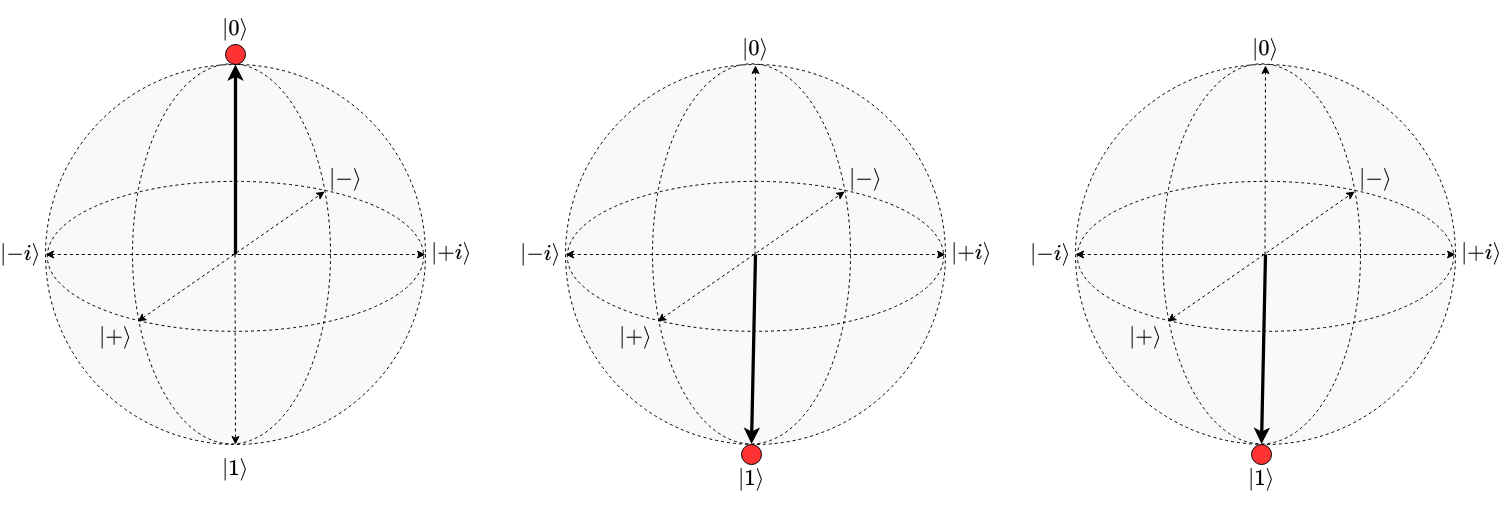
\includegraphics[width=0.94\linewidth]{body/ch4/figs/bloch-011}
	\caption[Bloch Sphere Representation of the Integer 3.]{A 3-qubit quantum state register can be represented on the surface of a Bloch sphere in the computational basis.}
	\label{fig:bloch-011}
\end{figure}
A unit circle, similar to the one implemented by Hlukhov, can be used to encode the positions of the unit vector based on the phase $\theta$ of a qubit as shown in figure \ref{fig:unit-circle}. 
\begin{figure}[!ht]
	\centering
	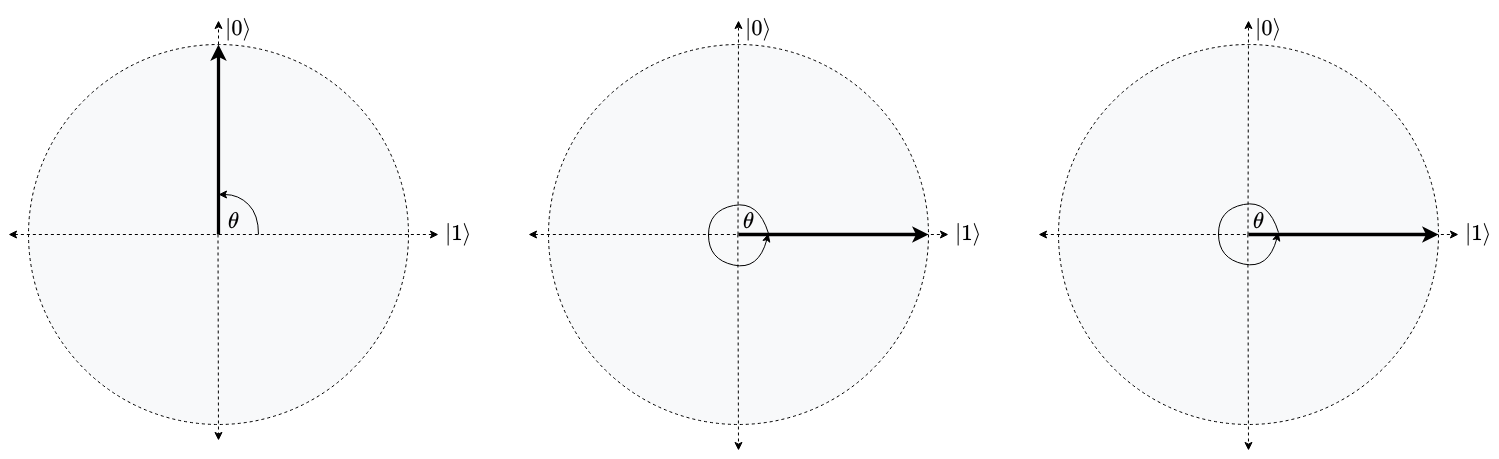
\includegraphics[width=0.94\linewidth]{body/ch4/figs/unit-circle-011}
	\caption[Unit Circle Graphical Representation of Integer 3.]{The 3-qubit register can be represented graphically on a unit circle. The phase $\theta$ of the quantum states can be used to minimise resource usage and memory.}
	\label{fig:unit-circle-011}
\end{figure}
Both representation afford the opportunity to represent the quantum state of qubits with respect to a single value corresponding to the phase $\theta$. Using the complex representation would require four values to represent one quantum state amplitude. However, noted in theoretical framework is that the normalised amplitudes can be expressed as the sinusoidal functions
\begin{align}\label{eqn:amplitude-sinusoids}
	\alpha_0	& = \sin(\theta)\\
	\alpha_1    & = \cos(\theta)
\end{align}
to produce the unit circle representation. The difference between the two graphical representations considered in the proposed design is that the Bloch sphere representation also requires storage of the relative phase of the qubit. This representation allows for more complex qubit operations that are not necessarily realisable on physical quantum computers. Furthermore, the spherical and circular representations can be used to display information about quantum states in a more intuitive manner to the user. 

\subsection{Methods for Initialising Qubits and Transmitting Quantum Information through a Quantum Channel \label{subsec:req-sim-gates}}

Satisfying the requirement for initialising qubits to a simple fiducial state is also considered from the perspective of the quantum interface. The model also considers qubit coupling to satisfy DiVincenzo's criteria. Users need to be able to initialise both physical and logical bits in the system.

In the proposed model, initialisation and transmission of well-characterised qubits is simulated using light from 8 GaAs LEDs to model Kimble et al. and Li et al.'s techniques for fabricating and capturing single-photon qubits using lasers, atoms and quantum dots \cite{turchette1995measurement, li2022control}. Physical qubits are coupled to one another using a collinear processor mapping in which the first qubit is coupled to the second qubit and the second qubit is coupled to both the third and fourth qubit. For the purposes of this design, the collinear mapping has no effect on the final result. Moreover, the system uses similar techniques to those employed in the QKD systems, such as the COW and Ent QKD systems, where a sender, Alice, transmits data to a receiver, Bob, through a quantum channel that exploit quantum entanglement. At the receiver of the quantum channel, InGaAs quantum dots and avalanche photodiode detectors are modelled using photoresistors in a BJT-based switching circuit. 

Preparation of qubits at Alice's location is modelled on the ARM-based microcontroller which toggles the LEDs to simulate propagation of flying qubits of weak coherent states from a CW laser as implemented in by the SECOQC project. Logical qubits in the proposed design are prepared in the computational basis and mapped to the physical qubits modelled by the LEDs, before transmission through the quantum channel. This is done through the linear qubit physical-to-logical qubit mapping scheme that is defined intrinsically on both the microcontroller and the FPGA in the SPQIS and QAES modules. For example, when an LED is \texttt{ON}, this could represent the $\ket{1}$ quantum state, while a LED that is \texttt{OFF} could represent the $\ket{0}$ states. Alternatively, a LED \texttt{ON} in a transmitted sequence could represent the position of 1 in the Hilbert space of the system as shown below. In both cases, probabilities can be preloaded to the devices from a pseudo-random number generator with a uniform distribution. 

\subsubsection{Quantum Channel Transmission Mode 1: Flying-Qubits in Binary Encoded Quantum Registers}

In the first method, each LED sequence represents a quantum register given by $\ket{q_{0}q_1\cdots q_{n-1}q_n}$. This method is illustrated in figure \ref{fig:qubit-mapping-method-1} where the quantum register $\ket{00010000}$ is directly reflected in the LED pattern in the sequence. Mathematically, this method for modelling qubit transmission through the quantum channel transfers the tensor product 
\begin{align}
	\ket{00010000}	 &  = \ket{0} \otimes \ket{0} \otimes \ket{0} \otimes \ket{1}\nonumber\\& \otimes \ket{0} \otimes \ket{0} \otimes \ket{0} \otimes \ket{0}\nonumber
\end{align} 
through a 1-1 mapping between quantum state $\ket{q_i}$ and LED $q_i$ in the sequence.
\begin{figure}[!ht]
	\centering
	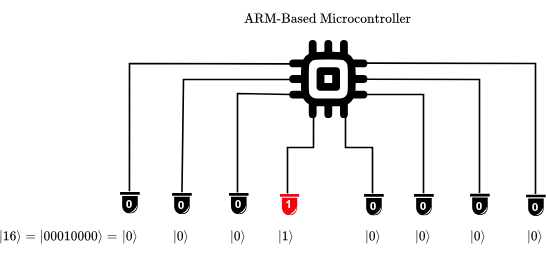
\includegraphics[width=\linewidth]{body/ch4/figs/qubit-mapping-method-1}
	\caption[Qubit Mapping Using LEDs for Direct Representation of the Computational Basis States $\ket{0}$ and $\ket{1}$.]{Illustrating the first method for initialising and transmitting quantum states directly as the tensor product $\ket{q_0} \otimes \ket{q_1} \otimes \cdots \ket{q_{n-1}}$. In this method, a single LED flash represents the basis vector $\ket{1}$ and a dim or \texttt{OFF} LED represents $\ket{1}$.}
	\label{fig:qubit-mapping-method-1}
\end{figure}
Using this direct qubit mapping technique provides a more straightforward way of modelling quantum computers with $n = 8$ qubits. For simulations of systems with less than 8 qubits, $n < 8$, the system must be able to discard or ignore parts of a transmitted LED sequence. For example, to represent a quantum system where $n = 3$, the only 3 LED out of 8 are required to transmit qubits in the quantum channel. Systems with $n > 8$ require multiple sequences to in order to transmit a full register. For example, to simulate the transmission of a system with $n = 12$ qubits, this method would require two and a half sequences to transmit the full register. In general, the number of sequences $s_1$, required to model an $n$-qubit transmission is given by
\begin{align}\label{eqn:number-of-sequences}
	s_1 & = n\cdot 2^{-3}
\end{align}
If $n$ is not a multiple of $2^3$, then the remainder from the division represents the portion of the LED sequence that can be discarded at the receiver. When a user initialises the system and sets input parameters related to the number of qubits, the system is should define the total number of LED sequences and the information that can be disregarded in the communication. 

This method was expected to provide a lower communication throughput and higher qubit transfer rates than the methods described below. In addition, given a system with $n$ bits, this method can transmit all the information about a quantum state using fewer LED sequences. Therefore, this method was expected to require less power than the other methods. From this analysis, it can be seen that power and the number of repetitions can be suitably employed as metrics for measuring the performance and communication efficiency of the quantum interface. 

\subsubsection{Quantum Channel Transmission Mode 2: Communicating with Quantum State Hilbert Spaces}
The second qubit initialisation and transmission technique also allows for a direct representation of qubit couplings as the quantum channel essentially transmits the topology of the Hilbert space of the quantum state in a pure form. This is because the 8 LED \texttt{ON} and \texttt{OFF} states can be directly mapped to the entries of the state column vector of a 3-qubit quantum register. For example, the column vector shown above for the computational basis representation of the integer 3 can be modelled using 8 LED bits as demonstrated in figure \ref{fig:led-qubit-mapping}. \\ 
\begin{figure}[!ht]
	\centering
	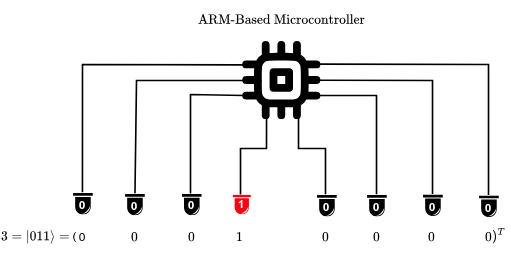
\includegraphics[width=1.0\linewidth]{body/ch4/figs/qubit-mapping-leds}
	\caption[Qubit Mapping Using LEDs to Represent 0s and 1s in Quantum State Vectors in the Computational Basis.]{A demonstration of a possible qubit mapping using the 8 LEDs to represent the 0s and 1s in the quantum state column vector that represents the integer $3_{10}$ in the computational basis as $\ket{011}_2$. The illustration shows \texttt{OFF} LEDs (0) in black, while the red colour illustrates an LED in the \texttt{ON} state. Note that, although the LED sequence is identical to the one shown in \ref{fig:qubit-mapping-method-1}, the information that is represented is not the same.}
	\label{fig:led-qubit-mapping}
\end{figure}
This method allows the quantum state to be transmitted as a vector through the quantum channel, offering a direct model of the quantum states that propagates through quantum channels as single-photons. To represent quantum computers with $n > 3$ qubits, multiple \texttt{ON} and \texttt{OFF} sequences can be programmed to ensure that all the $2^n$ matrices are displayed. Since each sequence can represent up to $8$ entries of the basis column vector, a factor of $2^3$ can be extracted from the $2^n$ entries to show that the number of LED sequences, $s$, that need to be performed to fully represent a quantum system with $n>3$ qubits is given by
\begin{align}\label{eqn:led-repetitions}
	s_2 & = 2^{n-3}
\end{align}
As a further illustration, consider the case where a 5-qubit quantum computer is being modelled. In this instance, the 8 LEDs have to flash 4 times in order to represent the basis column vector fully. This implies that the increasing the number of qubits in the system also increases the communication complexity and the throughput of the emulated system. Moreover, entangle qubits present a larger communication overhead in the quantum channel. This is due to the fact that entangled states come in EPR pairs, which require double the resources to represent each state of the pair. If qubits are entangle, Alice and Bob are required to share halves of the EPR states at the start of the communication protocol.

According to literature, these quantum states need to have sufficiently long enough decoherence times. For the proposed design, decoherence times of qubits is correlated to the duration of the \texttt{ON} and \texttt{OFF} LED pulses. Different pulse durations can be tested to simulate the effect of different decoherence times on the throughput and latency of a quantum communication system that is facilitated in the interface between a quantum computer and a classical computer. The communication protocol that handles the transfer of the bits requires a clear separation between signed, integer bits and mantissa bits. Since the modelled CW laser has large coherence times, the clocks on both the microcontroller and FPGA board can be used independently to control the emission and detection of simulated single-photon qubits. Tests can be conducted to find the optimal simulation of the decoherence of qubits based on the clock frequencies of the different boards. In an implementation of a quantum channel in a QKD network at the SECOQC project, TREL used a one-way weak pulse system that transmits optical pulses at a repetition rate of about $\SI{7}{\mega\hertz}$. In contrast, available microcontroller and FPGA clocks can operate at frequencies between or over $\SI{48}{\mega\hertz}$ to $\SI{133}{\mega\hertz}$, which is sufficient to model the operation of a quantum channel a the QKD network. 

LED sequences can be driven by the GPIO pins of the microcontroller. LED pulse sequences, whether representing the a 0s and 1s in the column vector or the phase, must be synchronised on the same clock to ensure that the LDR sensors on FPGA detect the pulse sequences in the correct window to avoid ambiguity in the quantum states. User need a way to initialise the qubits at the same time. Notably, the ARM-based model of the CW laser controller is not required to perform any computations. Quantum algorithms and quantum gate operations are performed on the FPGA only. To ensure security in models of quantum teleportation and key distribution, qubit paths in the quantum channel are occluded inside a tubular cases as illustrated in figure \ref{fig:led-to-ldr}, where each LED is directly aligned to the detection system connected to the FPGA such that one LDR can detect light from 1 LED.
\begin{figure}[!ht]
	\centering
	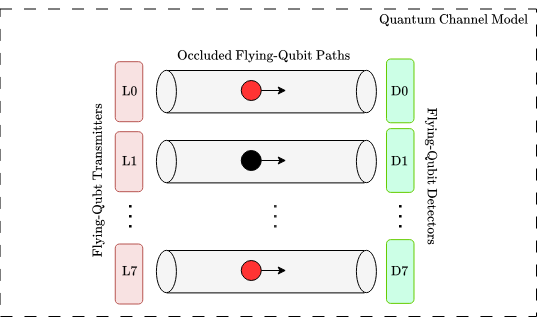
\includegraphics[width=1.0\linewidth]{body/ch4/figs/led-to-ldr}
	\caption[Illustration of the Security Measurements Implemented in the Quantum Communication Channel.]{An illustration of the occluding flying-qubits in order to prevent attacks from an eavesdrop. Moreover, in line with physical quantum computers, the user has no direct access to qubits in the entire emulated system except during initialisation and when performing measurements on the output.}
	\label{fig:led-to-ldr}
\end{figure}

When a measurement is performed on a qubit, it collapses to a classical bit according to the probabilities. This implies that the outputs from the FPGA quantum emulator should be able to represent qubits and classical bits on quantum and classical channels, respectively. Information about quantum state, for example, phase or probabilities, must be consistent on both platforms. Since the LEDs only represent the basis states, the communication protocol needs to include method of associating a probability or angle to each qubit. In this proposal, probabilities can be generated from a uniform distribution in MATLAB prior to starting the system. The generated probabilities can be preloaded on the microcontroller or stored in external memory on the FPGA.

\subsection{Flying Qubit Detection and Synchronisation of Classical and Quantum Systems \label{subsec:fqds-synch-requirements}}

The light from the LEDs propagates through the quantum channel through a model of a fibre link as implemented in the QKD systems explored in literature. Since the proposed design is for research purposes and modelling the operation of a quantum computer in laboratory settings, the short length of the modelled fibre link was not expected to contribute significantly to flying-qubit propagation delays. The design uses a series of 8 photoresistors, or LDRs, to simulate the use of single-photon InGaAs APD sensors for capturing flying qubits in the computational basis while ensuring that the quantum channel is secure. 

APDs are more sensitive devices that are used in specialised cases, whereas photoresistors are typically used as low cost photo sensitive elements. The aim of the photoresistor circuit is not to model the physical properties of APDs. Instead, the photoresistor circuit aims to model transmission of quantum information in the form of light. Due to their low-cost and sensitivity to light, photoresistors are suitable for modelling the conversion of quantum information from flying qubits to stationary qubits. 

In the proposed design, modelled flying-qubits are transmitted and recaptured within a detection window. If an LED is \texttt{ON} in the window, the resistance of the photosensors decreases, corresponding to the qubit state $\ket{1}$. If an LED is \texttt{OFF}, the resistance increases, corresponding to the state $\ket{0}$. Since the high resistance state corresponds to the $\ket{0}$, qubits are initialised in appropriately in the ground state on the quantum computer emulator. Photoresistors typically take time to transition between the high and low resistance states. This transition time between high and low resistance states was expected to contribute to communication delays, thereby affecting the overall communication efficiency of the model of the quantum channel. 

Furthermore, the transition time between resistance states directly affects the duration of the detection window. If the transmission time of the sensors is $t_s$, then the \texttt{ON} and \texttt{OFF} times of the LEDs, $\tau$, should be greater than $t_s$. To compensate for other errors and delays, an additional time $t_\epsilon$, is added to the on-and-off time to ensure that the total duration of the detection window is sufficiently long enough to capture data. By adjusting the on-and-off times, errors can be introduced into the system for perform quantum error correction experiments. 

To ensure that the detection window is initialised at the same time on the ARM microcontroller and the Xilinx FPGA, the proposed solution uses a \texttt{trigger} signal in a configurable bus as illustrated in figure \ref{fig:trigger}. The same line is used to allow the user to \texttt{enable} and \texttt{reset} the system in case they want to make changes to the input parameters. A different line, the \texttt{ack} signal, is used to allow the devices to communicate during the different stages of the communication protocol. The communication protocol depends on the format in which the qubits are transmitted through the quantum channel. If transmission mode 1 is used, then the first step in the communication protocol would require the source microcontroller to indicate to the FPGA emulator that the information is transmitted as pure quantum states. This can be accomplished by transmitting a 0 or 1 through the \texttt{async} line after the user has selected the qubit mapping at the source. 

\begin{figure}[!ht]
	\centering
	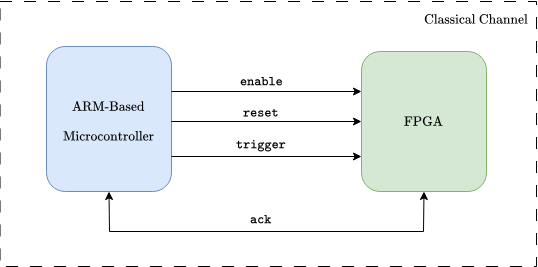
\includegraphics[width=1.0\linewidth]{body/ch4/figs/trigger}
	\caption[Illustrating the Classical Channel Between the ARM-Based Microcontroller and the FPGA.]{A \texttt{trigger}, \texttt{enable} and \texttt{reset} signal is transmitted through the bus between the microcontroller and FPGA. The \texttt{ack} signal is used at different stages of communication protocols to indicate when information has been transmitted.}
	\label{fig:trigger}
\end{figure}

Careful considerations were made in the design regarding minimum and maximum logic voltage levels and the maximum current that can be supported by the GPIO pins of the microcontroller and FPGA. To limit the collector current $I_C$ while maintaining the required voltage logic levels, the proposed electronic circuit for modelling qubit detection uses the photoresistors to divide the base voltage $V_B$ of a NPN type BJT. When the photoresistor is occluded, the BJT is in the cutoff region, and no current can flow. When light from the LEDs is incident on the photoresistors, the BJT is saturated and current can flow through the collector to the emitter. Therefore, current flows through the sensor when an LED indicates the quantum state $\ket{1}$. This feature of BJTs ensures that the resistance states, corresponding to the basis states, are well separated. Additionally, the maximum current through the BJT is determined by the gain. Therefore, the selection of the BJT depends on the current gain and the maximum current that is supported by the FPGA. 

Since flying qubits and their preparation are modelled using LEDs in the visible spectrum, an eavesdropper, Eve, can perform attacks simply by looking at the communication channel. Using a similar approach to the illumination-based method proposed by Lydersen et al. for preventing fake-attacks through background illumination of APDs, the proposed design uses an obscured quantum channel that prevents attackers from observing prepared quantum states or inducing false detections at the photosensors. By using an opaque fibre link, the model can securely transmit flying qubits from the source to the detectors. In addition, by covering the quantum channel, the model was expected to successfully transfer qubits with low transmission losses and a reduced false-detection rate from detection of lights in the environment. 

Overall, the electronic module modelling a quantum channel needs to be compatible with the peripherals on the FPGA board. FPGAs typically have female connectors for direct connection of peripheral module boards. Therefore, the quantum channel module is required to have male connectors. As mentioned, the output signal from the peripheral quantum channel module should conform to the LVCMOS 3.3V or LVTTL 3.3 logical conventions to improve resistance state detection precision \cite{diligent2011pmod}. On Xilinx FPGAs, the I/O pins generally have symmetrical $\SI{24}{\milli\ampere}$ source and sink capabilities \cite{diligent2011pmod}. In contrast, the drive strength of microcontrollers is generally less, typically in the range between $\pm\SI{5}{\milli\ampere}$ and $\pm\SI{10}{\milli\ampere}$) \cite{diligent2011pmod}. The proposed solutions uses the microcontroller to drive the emitter and receiver of the quantum channel model. The photoresistor circuit employs the Pmod Interface Type 1 interface for general purpose logic. Therefore, the GPIO pins on the microcontrollers should be configured as outputs while the Pmod GPIO pins on the FPGA should be set up as inputs. 

On the microcontroller, bit patterns on the LED circuit can be toggled using embedded C. On the FPGA, Verilog HDL code can suitab ... The use of appropriate delays is crucial for modelling the decoherence times of qubits and configuring the duration of a detection window. 

\subsection{Storing Qubits on the FPGA}

After a qubit is detected, the quantum state information needs to be stored on the FPGA according on the transmission method selected by the user at the start of an experiment. In the direct representation of qubits state, each qubit is detected and stored directly as a bit in memory in order to maintain the same sequence of qubits. This method allows for efficient retrieval and manipulation of qubits during emulation. The stored string of bits can be interpreted as the tensor product of the basis states. Each basis state can be store in the external memory of the FPGA along with the probabilities or phases associated with each state. 

At the end of the detection window, a digital signal is transmitted through the \texttt{ack} line from the microcontroller in the classical channel to the FPGA to indicate that transmission is complete. To further remove ambiguity in qubit states, the communication protocol transfers an additional bit through the \texttt{trigger} to enable the use of gray code for labelling the different properties of the qubit stream in a finite state machine. For example, if the \texttt{trigger} bit is zero and the states are not entangle, then the bit sequence 00 is transmitted to indicate to the emulated quantum computer that the qubit transfer is complete. If the quantum states are entangled, then the signal carrying 01 is transmitted to indicate that a Bell state measurement has been performed by Alice at the source.

Information about the quantum algorithm to be performed can also be encoded in the digital signals transferred through the classical net. Once the final \texttt{ack} signal is received, the FPGA can perform scalar multiplication of the state vectors with the preloaded probabilities. The output of the scalar product is stored in a different part of the FPGA memory to complete the initialisation of qubits on the emulated quantum computer. The total number of registers used in memory depends on the user defined parameters and the register widths depend on the number of mantissa bits in the fixed-point representation of phases and probabilities. 

The second quantum channel transmission mode which transfers the Hilbert space of a qubits was expected to require more registers to store quantum state data on the FPGA at the start of an experiment. For this method, the ground state Hilbert space of the $n$-qubit quantum register is preloaded in external memory along with the phases using a fixed-point representation. Similar to the previous method, the qubit stream is stored as a bit-string in the external memory of the FPGA. Once a signal indicating the end of a detection window is detected by the device, elements in the stored column vector of the ground state are updated with the correct amplitudes. 

Regardless of the transmission mode selected, software-based error detection mechanisms need to be enforced in the FPGA to check for inconsistencies in the received qubit states, particularly during quantum error correction experiments. The error detection mechanism needs to ensure that the stored qubits on the FPGA reflect the transmitted qubits accurately. Although more straightforward to implement, the first method was expected to require more clock cycles (and therefore more power) for storing the full description of a well-characterised qubit in memory since the quantum register is in the decomposed tensor product form. This is because the first method requires further processing before storing the complete column matrix of the qubit Hilbert space for further processing with quantum gate operations.

Most FPGAs offer various external memories, including DDR2 and DDR3 SDRAM as some of the common high-performance memory types for storing large amounts of data and enabling fast read and write operations through high-speed interfaces such as the advanced extensible interface (AXI4). Xilinx 7 series FPGAs use SLICEMs to implement function generators or LUTs as synchronous RAM registers called distributed RAM (DRAM) elements \cite{xilinx20167series}. DRAM modules provide asynchronous write capabilities and allow synchronous read operations to be implemented with a flip-flop in the same slice to improve the performance \cite{xilinx20167series}. 

RAM elements can be configured within a SLICEM to implement different combinations of ports and data widths. Using the single port configuration to perform storage operations on the quantum state representations could prove to be slow since synchronous writes and asynchronous reads are performed on the same address bus. More suitable distributed RAM configurations include the dual port, simple dual port and quad port configurations whose multiple ports can be used for synchronous writes and asynchronous reads of quantum state vectors. On the Xilinx 7 series FPGAs, maximum data transfer can be achieved using the quad port configuration which uses one port for synchronous writes and asynchronous reads, and three ports for asynchronous reads \cite{xilinx20167series}. In each case, all storage elements share in the distributed RAM share a common control signal clock (CLK), control enable (CE) and set/reset (SR). CE and SR signal are active high. To store quantum state information on the distributed RAM, storage elements can be forced into the state specified by the logic of the SR signal. 

To avoid using flip-flops which potentially requires more clock cycles for storing sensor data, SLICEM function generators can be configured as 32-bit shift registers such that each LUT can delay serial data from 1 to 32 clock cycles. Since the clocks rates of the FPGA and microcontroller are not the same, this method is more suitable since asynchronous FIFO I/O buffers can be used to facilitate read and write operations on the clock domain of the FPGA only. Using the first qubit transmission technique where the LED status indicates the computational basis state, photoresistor detection data can be stored in the FIFO as soon as they are detected. Since each detection is 8 bits, each clock cycle would store eight quantum states in a quarter of a 32-bit shift register on the FPGA. Figure \ref{fig:fifo-shift-register} illustrates the construction of a 32-bit shift register occupying a single LUT. Smaller shift registers can be built on Xilinx FPGAs by varying the address of LUT outputs corresponding to the desired width \cite{xilinx20167series}. For example, a 13 bit register can be configured by setting the address of the LUT output in the CLB slice to the 13th bit \cite{xilinx20167series}.
\begin{figure}[!ht]
	\centering
	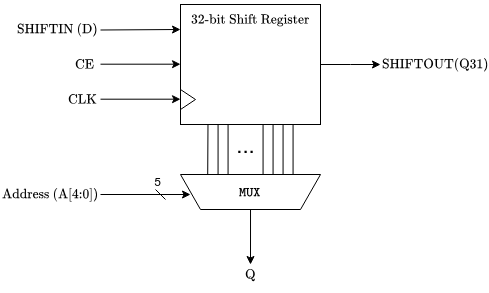
\includegraphics[width=0.85\linewidth]{body/ch4/figs/fifo-shift-register}
	\caption[Xilinx 7-Series 32-bit Shift Register.]{Xilinx 7-series FPGAs allow FIFOs to be implemented using the illustrated 32-bit shift register primitive. Write operations are synchoronous with the clock input (CLK) and the optional clock enable (CE). Shift registers are used to store sensor values in real-time. Shift registers allow dynamic reads through the LUT outputs labelled Q by varying the address \cite{xilinx20167series}. This feature is used later to specify the number of qubit quantum state vectors to be transferred to the distributed RAM.}
	\label{fig:fifo-shift-register}
\end{figure}

Using an asynchronous FIFO ensures that read and write operations of qubit detections can be written to the FIFO from the quantum channel circuit for different decoherence times. As the FIFO is read, qubit state vectors can be stored in distributed RAM elements. 

\subsection{Simulating Quantum Algorithms on a FPGA \label{subsec:req-sim-qualgorithms}}

The proposed design aims to emulate the following quantum algorithms and their associated quantum circuits:
\begin{enumerate}
	\item 
	Quantum Teleportation
	\item 
	Quantum Fourier Transform
	\item 
	Quantum Factoring Algorithm (Shor's algorithm)
	\item 
	Quantum Search Algorithm
\end{enumerate}
For each quantum circuit, a set of quantum gate operations is executed on the qubit matrix representations stored in the computational basis. Implementation of quantum gates depends on the hardware architecture of the FPGA. 

\subsubsection{Set of Universal Set of Quantum Gates}

The notion of \textit{clock time} in quantum computing is extended to the design of the FPGA-based quantum computer emulator in that the execution time of an experiment on the system is significantly influenced by the time it takes to execute  blocks. Literature shows that the execution time of single-qubit gate operations such as the Pauli gates in \ref{eqn:pauligates}, is negligibly small in comparison to execution times of multi-qubit gates such as the \texttt{CNOT} gate in \ref{eqn:cnotdef} and \ref{eqn:cnotmatrix}. A quantum gate of particular interest in the development of single-qubit gates is the Hadamard gate, since its output is a superposition of states. Based on the description of the quantum algorithms in chapter \ref{sec:ch2-conclusion}, the set of universal single and multiple qubit quantum gates that was expected to fulfil the requirements includes the:
\begin{itemize}
	\item 
	Pauli-X gate (\texttt{X})
	\item 
	Pauli-Z gate (\texttt{Z})
	\item 
	Hadamard (\texttt{H})
	\item 
	Controlled-R gate (\texttt{RNOT})
	\item 
	Controlled-NOT gate (\texttt{CNOT})
\end{itemize}
The identity gate \texttt{I} is implicitly included in the set since it leaves quantum states unchanged. As noted in the theoretical section, quantum gate operations on qubits represent tensor products and matrix multiplications. For example, an application of \texttt{X} gates to the initial quantum state register $\ket{010}$ is mathematically equivalent to the product
\begin{align}\label{eqn:3x-gates}
	X\ket{2}_{10} = X\ket{010}_{2}	& = X\ket{0}\otimes X\ket{1} \otimes X\ket{0}\nonumber\\
				& = \left(\begin{matrix}
					0 & 1\\
					1 & 0
				\end{matrix}\right) \cdot \left( \begin{matrix}
				1\\ 0
			\end{matrix}\right) \otimes \left(\begin{matrix}
			0 & 1\\
			1 & 0
		\end{matrix}\right) \cdot \left( \begin{matrix}
		0\\ 1
	\end{matrix}\right) \nonumber\\ & \otimes \left(\begin{matrix}
	0 & 1\\
	1 & 0
\end{matrix}\right) \cdot \left( \begin{matrix}
1\\ 0
\end{matrix}\right)\nonumber\\
& = \left(\begin{matrix}
	0 \\ 1
\end{matrix}\right)\otimes\left(\begin{matrix}
1 \\ 0
\end{matrix}\right)\otimes\left(\begin{matrix}
0 \\ 1
\end{matrix}\right)\nonumber\\
& = \ket{101}_{2} = \ket{5}_{10}
\end{align}
The equivalent quantum circuit representation for the above operation shown in figure \ref{fig:3-x-gates}. 
\begin{figure}[!ht]
	\centering
	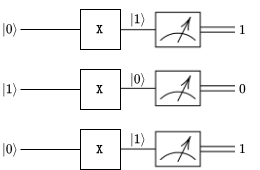
\includegraphics[width=0.85\linewidth]{body/ch4/figs/3-x-gates}
	\caption[Illustrating a Simple Bit Flip Using 3 \texttt{X} gates.]{Single-qubit quantum gates such as the \texttt{X} gate can be implemented directly in FPGA LUTs. This example illustrates a bit flip that would change the output of the LUT from 010 (or INIT[2] on a Xilinx 7-series FPGA) to 101 (INIT[5]).}
	\label{fig:3-x-gates}
\end{figure}

In this case, the data-width of the input and output quantum states is expected to remain the same. Therefore, if all the input and output relations are tabulated, a finite state machine can be used to represent quantum states in gray code to map the transformations for each value in a LUT. Multiple-qubit gates such as \texttt{CNOT} and \texttt{RNOT} gates can be stored directly in the distributed RAM as vectors. The control qubit and target qubits can be stored separately and used as input operands to multiplier and adder IP cores when performing controlled quantum gate operations. Equation \ref{eqn:generic-cnot} implies that memory usage for storing controlled gates of the form $\Lambda Q$ can be reduced by storing a template of the matrix operation with place holder values for the elements labelled $q_{11}$, $q_{12}$, $q_{21}$, $q_{22}$. Using a generic template could lead to potential increases in power usage as more clock cycles of the FPGA would be required to read the template from memory and construct the desired gate by changing the place-holder values.

Recall that to perform a unitary transformation on a $n$-dimensional Hilbert space, the quantum gate operator needs to be a vector space with $2^n \times 2^n$ dimensions. The proposed solution uses DDR SDRAM memory to resolve larger quantum gate operations instead of BRAMs on the FPGA fabric. An AXI manager interface to access data by communicating with vendor provided memory interface IP cores that allow asynchronous read and synchronous write interactions with the DDR SDRAM memory. Notably, DDR3 and DDR4 based RAMs operate at double the clock frequency, providing high data bandwidth, which is suitable for the high-throughput requirements involved in quantum gate operations. 

For example, to perform the \texttt{QFT} subroutine on the 3-qubit register $\ket{011}$, the $2^3 \times 2^3$ matrix demonstrated in equation \ref{eqn:qft-matrix} needs to be multiplied by the Hilbert space of the quantum state in the form
\begin{align}\label{eqn:qft-example-2}
	\texttt{QFT}\ket{011} = \nonumber\\ \frac{1}{\sqrt{8}}\left(\begin{matrix}
		1 & 1 & 1 & 1 & 1 & 1 & 1 & 1\\
		1 & \omega & \omega^2	& \omega^3	& \omega^4	& \omega^5	& \omega^6	&	\omega^7\\
		1 & \omega^2 & \omega^4	& \omega^6	& 1	& \omega^2	& \omega^4	&	\omega^6\\
		1 & \omega^3 & \omega^6	& \omega^1	& \omega^4	& \omega^7	& \omega^2	&	\omega^5\\
		1 & \omega^4 & 1	& \omega^4	& 1	& \omega^4	& 1	&	\omega^4\\
		1 & \omega^5 & \omega^2	& \omega^7	& \omega^4	& \omega	& \omega^6	&	\omega^3\\
		1 & \omega^6 & \omega^4	& \omega^2	& 1	& \omega^6	& \omega^4	&	\omega^2\\
		1 & \omega^7 & \omega^6	& \omega^5	& \omega^4	& \omega^3	& \omega^2	&	\omega^1
	\end{matrix}\right) \left(\begin{matrix}
	0 \\ 0 \\ 0 \\ 1 \\ 0 \\ 0 \\0 \\0 
\end{matrix}\right)
\end{align}
where $\omega = e^{2\pi/8}$. Provided that the elements of the \texttt{QFT} are calculated before pre-loading them in memory, performing the above operation would require 65 multiplications and 64 additions to produce the output. To perform multiplication operations on the proposed hardware, fixed-point parallel multipliers and constant-coefficient multipliers for two's complement signed or unsigned data can be generated using IP cores in FPGA design tools such as Xilinx Vivado for Xilinx FPGAs or Quartus Prime for Intel FPGAs. The total number of multipliers and adders required to model a unitary transformation on a $n$-qubit quantum system can be derived from the above example by observing that the $n$-qubit output $\ket{\psi_f}$ is given by the sum of the product between elements $u_{ij}$ of the unitary matrix $U$ and the elements in the initial quantum state column vector $\psi$, i.e.,
\begin{align}\label{eqn:multipliers+adders}
	\ket{\psi_f}	& = \sum_{j = 1}^{2^n} u_{ij} \cdot \psi_{j}~,~\text{for}~i=1,2,...,2^n
\end{align}
This implies that for quantum gate emulations of $n$-qubit systems:
\begin{itemize}
	\item 
	$2^n$ multipliers are required to handle the product of each element $u_{ij}$ of the $2^n \times 2^n$ unitary transform $U$, with the corresponding $n$ elements from the quantum state vector
	\item
	$2^n - 1$ adders are required to handle the compute the final value of each entry in the state vector of the output state $\ket{\psi_1}$
\end{itemize}
In this design, the proposed hardware architecture performs multiplication operations in pipelined stages. Multiplier pipelines take advantage of the inherent parallelism in FPGA architectures which have dedicated resources for performing fixed-point multiplication such as slice logic and DSP slices. For multiplication of large matrices, the number of pipeline stages needs to selected to satisfy the latency and performance requirements. Parallel multiplication can be optimised by reducing DSP sliced base multiplier utilisation by using an amalgamation of slice logic and dedicated multiplier primitives \cite{xilinx20167series}. The area of LUT-based multipliers such as the ones used for single-qubit gates can be optimised by ensuring that both input operands are unsigned, and that both input operands are smaller than 16 bits. Application of pipelined stages to perform quantum gate operations was expected to introduce latency effects to the system. In this paper, optimal pipelining was achieved using the pipeline registers inside DSP slices of multiplier cores as shown in figure \ref{fig:dsp-opt-pipeline} \cite{xilinx2014multiadder}.
\begin{figure}[!ht]
	\centering
	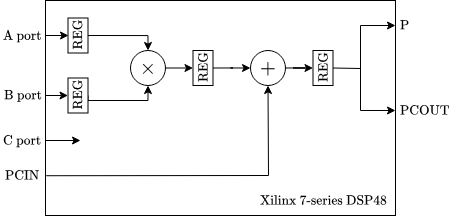
\includegraphics[width=0.80\linewidth]{body/ch4/figs/dsp-opt-pipeline}
	\caption[Illustrating Xilinx 7-Series FPGA DSP48 for Performing Matrix Products Associated with Quantum Gate Operations.]{An illustration of the DSP48 slice implementation which can be used to perform quantum gate operations in the computational basis.}
	\label{fig:dsp-opt-pipeline}
\end{figure}

Since detected quantum states are stored in $m$-bit shift registers, multiplier and adder cores need to support inputs ranging from 1 to $m$-bits wide and outputs ranging from 1 to $2m$ bits wide. The output data width needs to be twice the width of the inputs because multipliers typically produce outputs with larger values that require wider registers to prevent bit overflow errors. Figure \ref{fig:xilinx-vector-multiply} shows an example of a simple vector multiply block with bit staggering. Bit staggering is used to achieve data alignment by ensuring that all inputs are right-justified when passed to the operators inside a multiplier core. Implementation of bit staggering in the architecture ensures that the core works for single or multiple DSP slice applications. Outputs from the different multipliers in the pipeline are cascaded using the \texttt{PCIN} and \texttt{PCOUT} ports.
\begin{figure}[!ht]
	\centering
	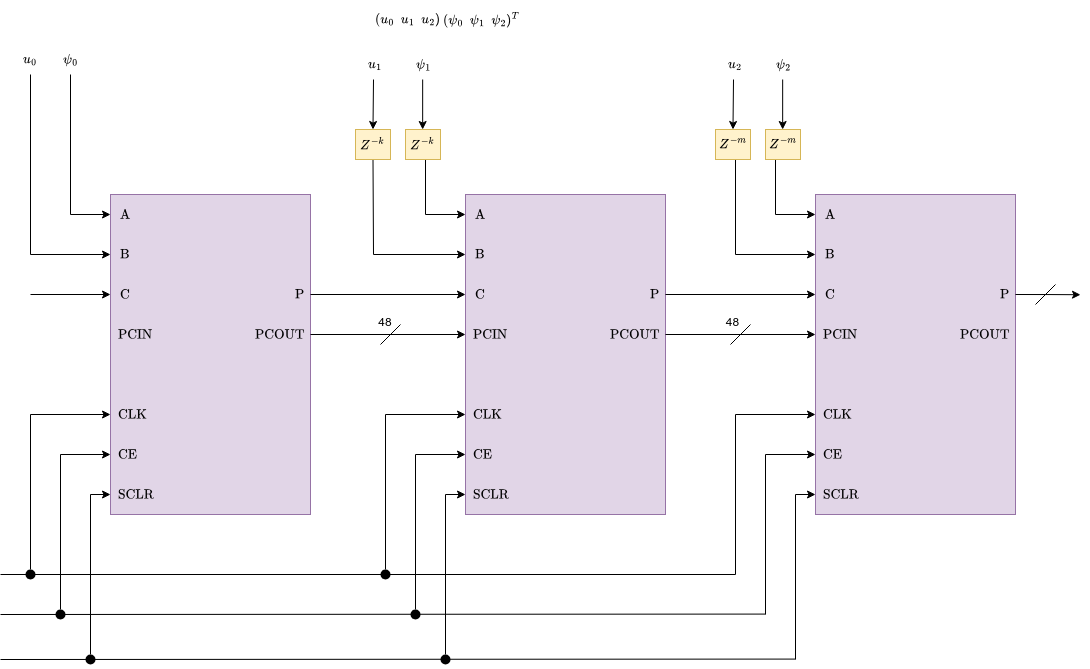
\includegraphics[width=\linewidth]{body/ch4/figs/xilinx-vector-multiply}
	\caption[Simple Vector Multiply Block using the LogiCORE IP Multiply Adder.]{A simple vector multiply for all DSP slice implementations of the Multiply Adder IP core in AMD Vivado and Xilinx 7-series FPGAs \cite{xilinx2015multiplier}. The example shown is implemented to multiply a single row in the unitary matrix of a quantum circuit with the column vector of the quantum state. The output of each multiplication is stored in pipeline registers of DSP slices.}
	\label{fig:xilinx-vector-multiply}
\end{figure}

Constant-coefficient multipliers, which are of crucial for computing products of basis vectors and their normalised amplitudes, can be constructed from distributed memory, block memories, or embedded multipliers \cite{xilinx2015multiplier}. The final output of the FPGA system corresponds to the output of the coefficient multipliers. This output is stored in the distribute RAM transferred to the UIS system, where it can be displayed to the user on the 7 segement display. In the proposed design, quantum gate errors were only considered to the extent of loss in precision due to the use of a fixed-point number scheme.  

\subsubsection{Quantum Teleportation Design Considerations for Hardware Emulation}

Quantum algorithms and quantum circuits are defined implicitly in the data paths, multipliers and adders in the pipeline. Since the pipeline stages use registers, the emulation cannot satisfy the no cloning theorem of qubits in the model as the classical bits that represent quantum states are duplicated for various reasons throughout the implementation. 

The aim of quantum teleportation is to verify the operation of the quantum channel in the context of a QKD network. In that sense, the quantum teleportation algorithm can also be interpreted as a qubit transfer protocol between the classical computer at the source and the quantum computer at the network edge. Furthermore, quantum teleportation circumvents the no cloning constraint on which prevents qubits from being duplicated. This is done by transfer the quantum state to a qubit in an entangled pair across the quantum channel using results from measurements of classical bits.

Literature shows that for Alice to convey $n$-qubits of information to Bob, at least $\lceil n/2\rceil$ qubits must be transmitted and both parties must share an entangled state prior to the initialisation of the communication channel. Requirements for performing the quantum teleportation to transmit key string $x$ can be derived from Cleve et al.'s observation that if the source transmits $n$ qubits to the photosensors, after both parties have shared prior entangled states, then at most $2n$ bits can be stored in the shift registers. If no prior entangled state information is stored, then each qubit sequence that is transmitted produces at most $n$ classical bits. The proposed design focuses on the case where prior entanglement information is shared between both parties.

In the first qubit transmission mode, if asynchronous writes to the FIFO macros are performed on a clock edge, then twice as many clock cycles are required to write sensor data to shift registers in the case where prior entangled state information has been shared. In the case where prior state information has not been shared, $1$ clock cycle would required for every 3 qubits in the system as shown in equation \ref{eqn:number-of-sequences}. Handshaking flags can be transmitted through the bus in the classical channel between the microcontroller and FPGA as previously described. The handshaking signals correspond to the classical measurements in the quantum circuit depicted in figure \ref{fig:quantum-teleportation-circuit}. The quantum gate operation that Bob needs to perform on their half of the EPR pair depends on the signal transmitted through the classical channel in the quantum interface as shown in table \ref{tab:teleportation-table}.

\begin{table}[ht!]
	\centering
	\caption[Table Showing Possible Classical Outputs and Required Quantum Gates for the Quantum Teleportation Circuit.]{Table showing possible classical outputs and the sequence of quantum gates that Bob is required to perform in order to recover the original quantum state at Alice's location.}
	\label{tab:teleportation-table}
	\begin{tabular}{ |c|c|c| } 
		\hline
		\textbf{Classical Output} & \textbf{Gate 1} & \textbf{Gate 2}\\ 
		\hline
		$(00)_2$ & \texttt{I} & \texttt{I} \\ 
		\hline
		$(01)_2$ & \texttt{X} & \texttt{I} \\ 
		\hline
		$(10)_2$ & \texttt{Z} & \texttt{I} \\ 
		\hline
		$(11)_2$ & \texttt{X} & \texttt{Z} \\ 
		\hline
	\end{tabular}
\end{table}

Quantum gates that are involved in the quantum teleportation protocol include the \texttt{CNOT}, \texttt{H}, \texttt{X}, and \texttt{Z} gates as illustrate in the quantum circuit in figure \ref{fig:quantum-teleportation-circuit}. 
\begin{figure}[!ht]
	\centering
	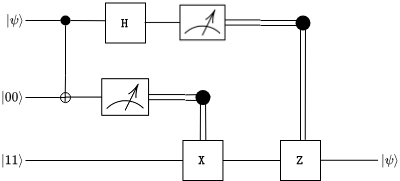
\includegraphics[width=\linewidth]{body/ch4/figs/quantum-teleportation-circuit}
	\caption[Quantum Circuit of the Quantum Teleportation Protocol.]{The quantum teleportation procedure implements \texttt{CNOT}, \texttt{H}, \texttt{X}, and \texttt{Z} gates in a sequence represented by the quantum circuit. The classically controlled quantum gate operations applied in this circuit correspond to the case where Alice measures bit sequence $(11)_2$.}
	\label{fig:quantum-teleportation-circuit}
\end{figure}

The two single gate operations are performed by Bob on the FPGA while the \texttt{CNOT} is performed at the source on the message qubit and one half of the entangle pair. In the proposed model design, the output of the \texttt{CNOT} gate transmitted as is and the matrix operation is not performed on the microcontroller. The result of Alice's state measurement is carried in the \texttt{trigger} and \texttt{ack} signals as a classical two-bit string. In the last stage of the protocol, Bob performs the single-gate operations depending on the classical bits and qubits transmitted from the source to effectively complete the transmission of the key $x$ as qubits. 

The quantum teleportation protocol and overview of required resources are summarised below:
\begin{enumerate}
	\item
	Alice and Bob one half of a previously prepared EPR pair. The qubit at the source is stored as a bit pattern on the microcontroller while Bob's half is stored in the external memory on the FPGA. In the quantum channel circuit, entangle qubits are represented by toggling the LED bit pattern between both qubits in the EPR pair. The FPGA only responds to half of the signal, although qubit detections from the photosensors are not stored during this process.
	\item 
	Alice performs a Bell state measurement to entangle the key $x$ with the entangled half of the EPR pair at the source. The output is transmitted in the \texttt{trigger} signal from the source microcontroller to the end-point FPGA.
	\item 
	Bob performs a series of single-qubit quantum gate operations to recover the key $x$. The output is displayed on the 7 segment display to determine if the transfer was successful.
\end{enumerate}

The proposed implementation uses a finite state machine (FSM) to emulate the quantum teleportation algorithm. Each state in the FSM is mapped to logic cells for emulating single-bit quantum gate operations 
\subsubsection{Simulating the QFT Transform Quantum Circuit}

The QFT can be implemented as an algorithm or a subroutine in the quantum factoring algorithm.In other words, the QFT behaves like a quantum gate, described by the product expansion in the computational basis and the matrix in \ref{eqn:qft-matrix}. 

As a standalone algorithm, the QFT takes in $n$ inputs corresponding and performs a series of quantum gates as shown in figure \ref{fig:nielsen-qft}. To emulate the \texttt{QFT} quantum circuit, vector multiplication are performed and outputs are stored in pipeline registers as illustrated in figure \ref{fig:qft-pipeline} below.
\begin{figure}[!ht]
	\centering
	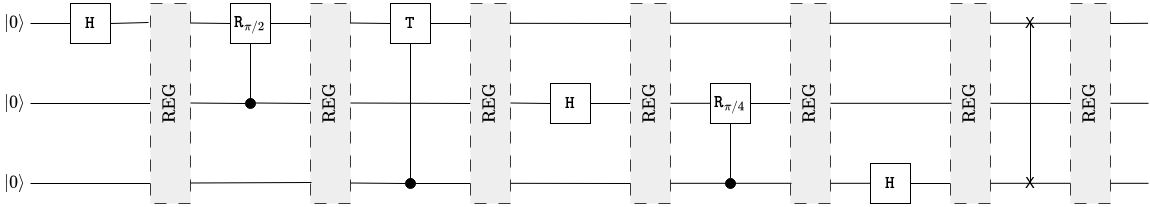
\includegraphics[width=1.0\linewidth]{body/ch4/figs/qft-pipeline}
	\caption[Illustrating the Implementation of DSP Pipeline Registers for Performing the QFT in the QAES.]{Pipeline registers are used to store intermediate results between gate operations. The final output of the quantum circuit is stored in the distribute RAM.}
	\label{fig:qft-pipeline}
\end{figure}

The pipeline can be summarised in the following pseudocode.
\begin{center}
	\textbf{Algorithm: 3-Qubit QFT}
\end{center}
\textbf{Inputs}: 3 qubits $\ket{j_1}$, $\ket{j_2}$, $\ket{j_3}$ initialised to $\ket{0}$\\
\textbf{Outputs}: 3 qubits $\ket{k_0}\ket{k_1}\ket{k_2}$\\
\textbf{Runtime}: $\mathcal{O}(\log_2 N)$

\fbox{%
	\begin{varwidth}{\dimexpr\linewidth-2\fboxsep-2\fboxrule\relax}
		\begin{algorithmic}[1]
			\Procedure{QFT}{$\ket{j_0}$, $\ket{j_1}$, $\ket{j_2}$}
			\State \ \ \ \ //apply Hadamard gate on first qubit
			\State \ \ \ \ \texttt{H} ($\ket{j_0}$); \\
			
			\State \ \ \ \ //apply controlled-$\texttt{R}_{\pi/2}$ with control qubit ~~~~~ $\ket{j_0}$
			\State \ \ \ \ \texttt{controlled\_R} ($\ket{j_1}$, ($\pi/2$, $\ket{j_0}$));\\
			
			\State \ \ \ \ //apply controlled-$\texttt{R}_{\pi/4}$ with control $\ket{j_0}$
			\State \ \ \ \ \texttt{controlled\_R} ($\ket{j_2}$, ($\pi/4$, $\ket{j_0}$));\\
			
			\State \ \ \ \ //apply Hadamard gate on second qubit
			\State \ \ \ \ \texttt{H} ($\ket{j_1}$); \\
			
			\State \ \ \ \ //apply controlled-$\texttt{R}_{\pi/2}$ with control qubit $\ket{q_1}$
			\State \ \ \ \ \texttt{controlled\_R} ($\ket{j_2}$, ($\pi/2$, $\ket{j_1}$));\\
			
			\State \ \ \ \ //apply Hadamard gate on third qubit
			\State \ \ \ \ \texttt{H} ($\ket{j_2}$); \\
			
			\State \ \ \ \ //swap qubits 1 and 3
			\State \ \ \ \ \texttt{swap} ($\ket{k_2}$, $\ket{k_0}$);\\
			
			\State \ \ \ \ \textbf{return} $\ket{k_0}\ket{k_1}\ket{k_2}$;\\
			
			\State \ \ \ \ //reset all qubits:
			\State \ \ \ \ \texttt{reset} ($\ket{j_0}$, $\ket{j_1}$, $\ket{j_2}$);
			\EndProcedure
		\end{algorithmic}
	\end{varwidth}% 
}

The pipeline registers store the data after executing each function in the pseudocode. From the above, it can be seen that 9 pipeline registers are required to perform the 3-qubit QFT. The output of the QFT represents qubits in the Fourier basis state $\ket{+}$ and $\ket{-}$, which can be used to represent the output quantum register $\ket{k_0 k_1 k_2}$ graphically as shown in figure \ref{fig:fourier-basis}. 

\subsubsection{Quantum Factoring Algorithm}

As shown in section \ref{subsubsec:q-shors-algo}, the quantum factoring algorithm applies principles of phase estimation using the inverse QFT to determine the period of an integer. This is useful for cracking the RSA public-key encryption pattern which generates a public-private key pair using two large prime numbers $p_1$ and $p_2$. Cracking the RSA pattern involves factorising a given large prime product $N = p_1 p_2$ in order to calculate the private key in the pair. The aim of the proposed design is to factor the integer $N = 21$ into the prime factors 3 and 7 using Shor's factoring algorithm. 

Given the integer $N$ to be factored, Shor's algorithm begins by choosing a random integer $x$ less than $N$ and coprime to $N$. Then, the algorithm finds the order $r$ of $N$ such that $x^r \equiv1\left(\text{mod}~N\right)$. The number of qubits $n$ is 
\begin{align}\label{eqn:shor-required-bits}
	n	& = \lceil \log_2 N\rceil
\end{align}
To factor the number $N = 21$, a total of 5 qubits is required to perform the operation. Three qubits form the control register and the other two qubits form part of work register. The inverse QFT, which is equivalent to applying the QFT circuit in reverse, is used to change to transform the first qubit register to the computational basis after applying Hadamard gates to each qubit.
\begin{figure}[!ht]
	\centering
	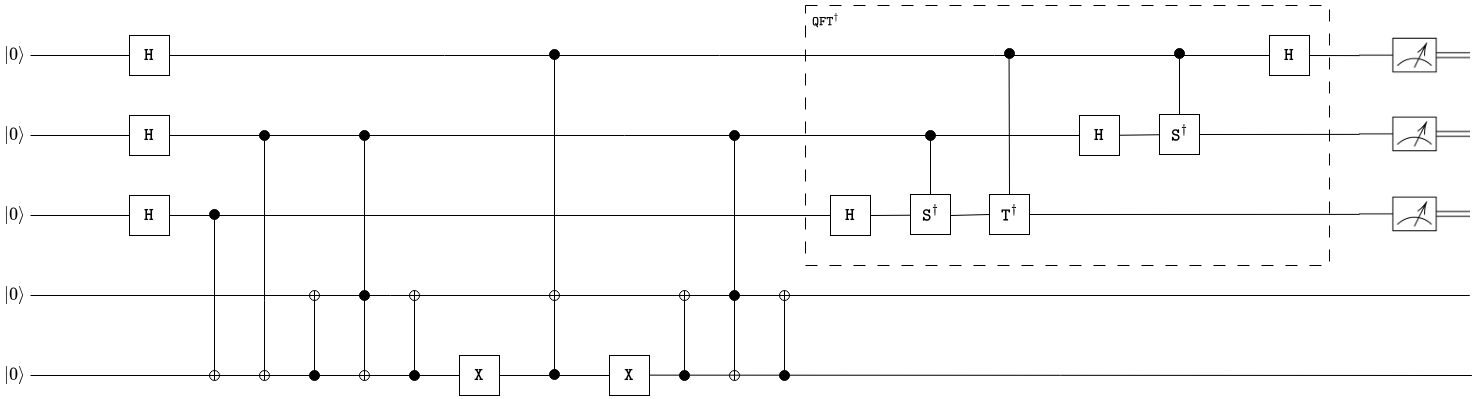
\includegraphics[width=1.0\linewidth]{body/ch4/figs/quantum-factoring-algorithm}
	\caption[Quantum Circuit Representation of the Emulated Quantum Factoring Algorithm for $N = 21$ and $a=4$.]{Showing the 5-Qubit quantum circuit for factoring $N=21$ and $x=4$  which applies the inverse QFT ($\texttt{QFT}^\dagger$) \cite{skosana2021demonstration}. The expected order of $N$ when $x = 4$ is $r$, which can be extracted from the output of the control register given by $2^n s/r$, where $s \in \mathbb{Z}$ is randomly assigned according to the measurement of the control register outputs.}
	\label{fig:quantum-factoring-algorithm}
\end{figure}

In this paper, simulation of the quantum factoring or (Shor's) algorithm for solving the order-finding problem is performed in relation to the quantum circuit shown in figure \ref{fig:quantum-factoring-algorithm}. When fully expanded, the quantum circuit shows that to successfully emulate the quantum factoring algorithm for $N = 21$ with an initial guess of $x = 4$, the system requires:
\begin{itemize}
	\item 
	25 \texttt{CNOT} gates
	\item 
	8 Hadamard gates
	\item 
	2 explicit \texttt{X} gates
	\item 
	2 controlled-$\texttt{R}_{\pi/2}$ gates
	\item 
	13 controlled-$\texttt{R}_{\pi/4}$ gate
\end{itemize}
Similar to the implementation of the QFT algorithm above, the quantum circuit is pipeline to store the state of the simulated qubits after each quantum gate operation. The circuit depth of Shor's algorithm is high due to the large number of quantum gates required to perform the procedure. This implies that the emulated quantum circuit also long critical path on the FPGA fabric, which leads to high latency and reduced performance. Additionally, storage, latency and power requirements are increased by pipelining the execution of the algorithm. Therefore, emulation of the quantum factoring algorithm for small integers such as $21$ is not expected to offer performance gains over PC-based simulations of the quantum factoring algorithm. 

In this implementation, the possible quantum states of the working register are encoded as follows:
\begin{align}\label{eqn:shor-work-register}
	\ket{1}_{10} \rightarrowtail \ket{00}_{2}\nonumber\\
	\ket{4}_{10} \rightarrowtail \ket{01}_{2}\nonumber\\
	\ket{16}_{10} \rightarrowtail \ket{11}_{2}
\end{align}
so that instead of evaluating $4^r~\text{mod}~21$, the quantum algorithm evaluates $\log_4(4^r~\text{mod}~21)$ \cite{skosana2021demonstration}. Given that $x = 4$, possible values of $r$ can be calculated from
\begin{align}
	4^0	& = 1~\mod 21\nonumber\\
	4^1	& = 4~\mod 21\nonumber\\
	4^2	& = 16~\mod 21\nonumber\\
	4^3	& = 1~\mod 21\nonumber\\
\end{align}
which shows that the period of $N = 21$ is 3 \cite{skosana2021demonstration}. Measurement of the control register output yields a probability distribution with peaks that correspond to values of $2^n \sigma/r$, where $\sigma$ is a randomly assigned number associated with measurement probabilities.

\subsubsection{Emulation of Grover's Algorithm}

The aim of the quantum search algorithm, or Grover's algorithm, is to find the solution $a$ of a function $f(x)$ that produces an outcome of 1. This can be used to find the index of an item in a database that matches given criteria labelled $x_0$. As mentioned in section \ref{subsubsec:q-search-algo}, the main advantage of using the quantum search algorithm is that it performs the entire search of a $N$-entry database in $\mathcal{O}(\sqrt{N})$, compared to sequential classical algorithms which perform the search $\mathcal{O}(N)$ time. 

For this implementation of the quantum search algorithm, a database with $N = 4$ entries as shown in table \ref{tab:grover-entries} where each item is indexed from 0 to 3. This implies that the emulated quantum computer only needs to represent two qubit registers in the hardware. 

\begin{table}[ht!]
	\centering
	\caption[Table Showing Indices and their Associated Strings for Performing the Quantum Search Algorithm.]{Table of two-qubit registers indices and their associated strings for performing the quantum search algorithm (QSA).}
	\label{tab:grover-entries}
	\begin{tabular}{ |c|c|c| } 
		\hline
		\textbf{Index} & \textbf{Name} & \textbf{QSA Output}\\ 
		\hline
		$\ket{00}_2$ & Kestrel & $\ket{00}_2$ \\ 
		\hline
		$\ket{01}_2$ & Kite & $\ket{00}_2$ \\ 
		\hline
		$\ket{10}_2$ & Harrier & $\ket{00}_2$ \\ 
		\hline
		$\ket{11}_2$ & Goshawk & $\ket{11}_2$ \\ 
		\hline
	\end{tabular}
\end{table}

Figure \ref{fig:grovers-circuit} shows the quantum circuit representation of the quantum search algorithm which consists of:
\begin{itemize}
	\item 
	6 Hadamard gates
	\item 
	2 Pauli-Z gates
	\item 
	2 Controlled-\texttt{Z} gates (\texttt{CZ})
\end{itemize}
\begin{figure}[!ht]
	\centering
	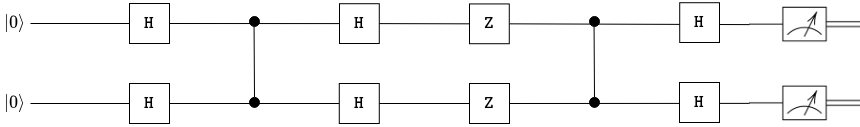
\includegraphics[width=1.0\linewidth]{body/ch4/figs/grovers-circuit}
	\caption[Quantum Circuit for Finding the Index of an Entry in a Database.]{The quantum circuit representation of the quantum search algorithm for finding the element in the index corresponding to the state $\ket{11}$.}
	\label{fig:grovers-circuit}
\end{figure}
The controlled-\texttt{Z} gates plays the role of the oracle in the Grover's iterative. Using the quantum information system equivalent of a truth table as shown in \ref{tab:controlled-z}, the outputs of the this two-qubit input gate can be seen more clearly. In the case where the input to the \texttt{CZ} gate is $\ket{11}$, the phase of the qubit is flipped as illustrated by the unit circle representation of the two-qubit register in figure \ref{fig:grover-phase-flip}.
\begin{figure}[!ht]
	\centering
	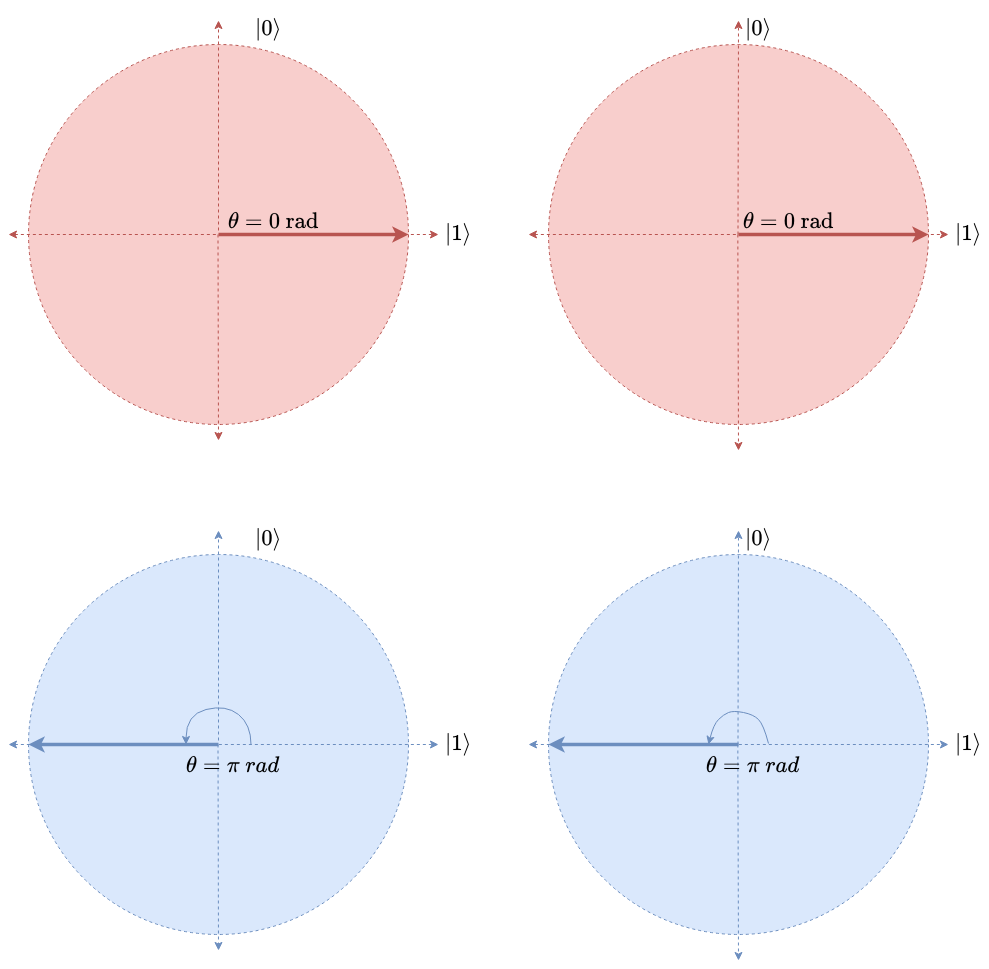
\includegraphics[width=1.0\linewidth]{body/ch4/figs/grover-phase-flip}
	\caption[Graphical Representation of the Controlled-Z Gate Applied in the Quantum Oracle of Grover's Search Algorithm.]{A unit circle representation of the application of the \texttt{CZ} gate to a quantum register which has an original state of $\ket{11}$ depicted in red. The expected output in this case is  $-\ket{11}$ depicted in blue.}
	\label{fig:grover-phase-flip}
\end{figure}
\begin{table}[ht!]
	\centering
	\caption[Table Showing the Input-and-Output Relationship of the \texttt{CZ} Gate in a Two-Qubit System.]{Input-and-output relationship for \texttt{CZ} gate shown as a quantum truth table.}
	\label{tab:grover-phase-flip}
	\begin{tabular}{ |c|c|c|c| } 
		\hline
		\textbf{Input} & \textbf{Control} & \textbf{Target} & \textbf{Output}\\ 
		\hline
		$\ket{00}_2$ & $\ket{0} $& $\ket{0}$ & $\ket{00}_2$  \\ 
		\hline
		$\ket{01}_2$ & $\ket{0}$ & $\ket{1}$ & $\ket{01}_2$ \\ 
		\hline
		$\ket{10}_2$ & $\ket{1}$ & $\ket{0}$ & $\ket{10}_2$ \\ 
		\hline
		$\ket{11}_2$ & $\ket{1}$ & $\ket{1}$ & -$\ket{11}_2$ \\ 
		\hline
	\end{tabular}
\end{table}
The corresponding high-level description for implementing the \texttt{CZ} gate using MATLAB matrix operations is given by
\begin{align}
	\left(\begin{matrix}
		1	 &	0	& 0 & 0\\
		0	 &	1	& 0 & 0\\	
		0	 &	0	& 1 & 0\\
		0	 &	0	& 0 & -1\\	
	\end{matrix}\right)\cdot\left(\begin{matrix}
	0 \\ 0 \\ 0 \\ 1
\end{matrix}\right)
\end{align}
The quantum circuit needs one iteration to find the solution, regardless of the position of the entry in the database. For demonstration purposes, the algorithm is implemented to find the index corresponding to the state $\ket{11}$. This result corresponds to the classical output registers at the end of a single iteration of the illustrated quantum circuit.

The proposed application of the search algorithm has a low circuit depth compared to the application of Shor's factoring algorithm as described in the previous subsection. A lower circuit depth indicates lower latency when emulating the algorithm in the fabric of the FPGA. In this paper, results of the execution of the quantum search algorithm are compared to the execution time of a sequential search algorithm that finds uses simple conditional statements to determine find $x_0$. 
 
\subsection{Design Tools and Workflow}

The following shows the design flow of the FPGA emulated quantum computer and quantum interface, including some of the tools used in the development of the integrated system.  

To initialise qubits and model laser pulses through LED status changes, the proposed design uses the ARM-based STM32F051C6 microcontroller due to its simple architecture and multiple GPIO pins for generating the required signals for driving LEDs as seen in figure \ref{fig:stm32-devboard}. The STM32 processor is a 32-bit processor which offers enhanced system debug with breakpoint and trace capabilities, as well as low power consumption and platform security. 
\begin{figure}[!ht]
	\centering
	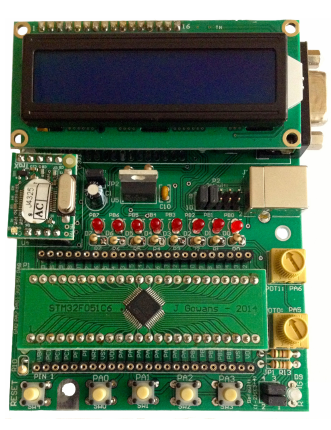
\includegraphics[width=0.30\linewidth]{body/ch4/figs/stm32-devboard}
	\caption[Image of the UCT STM32F0 Development Board Used to Model the Behaviour of a Laser-Based Flying-Qubit Transmitter.]{Image of the UCT STM32F0 daughter board used to model the behaviour of a laser-based flying-qubit transmitter in the SPQIS and FQDS subsystems}.
	\label{fig:stm32-devboard}
\end{figure} 

The first iteration of the electronic circuit for modelling the quantum channel is built on a breadboard. Following verification of output voltages and currents, the final design was built on veroboard due to its low cost.

Quantum circuits are emulated on the Nexys A7 FPGA board (shown in figure \ref{fig:nexys-a7}) which is designed around the Xilinx Artix-7 FPGA family. The board was selected for its ready-to-use digital circuit, versatile interfaces and vast resources which can reduce development time. Additionally, the board is compatible with the AMD Vivado design suite which provides a graphical representation of the circuit and IP cores that can be used to map quantum algorithms to hardware in the synthesis stage of development. Vivado also offers automatic optimisations of placement, routing and clock frequencies in the hardware design. 
\begin{figure}[!ht]
	\centering
	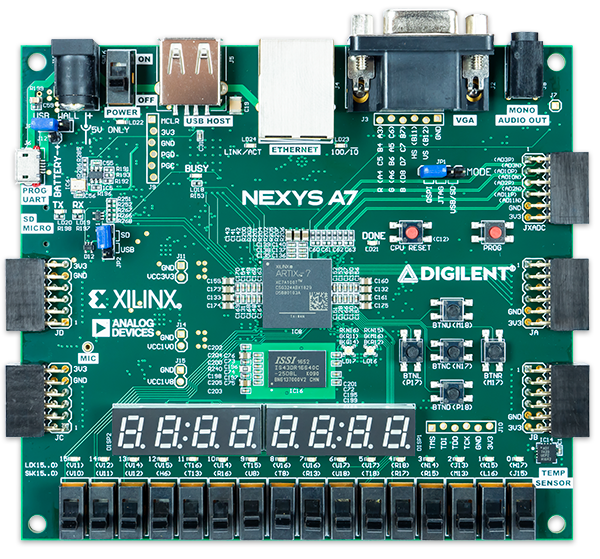
\includegraphics[width=0.55\linewidth]{body/ch4/figs/nexys-a7}
	\caption[Nexys A7 Board based on the Xilinx 7-Series FPGAs.]{Image of the Nexys A7 board which is based on the Artix-7 series \cite{diligent2024nexysa7}.}
	\label{fig:nexys-a7}
\end{figure}

Before synthesis, algorithms are modelled and tested using MATLAB, Simulink and SystemVerilog simulations. Python simulations of quantum circuits using the Qiskit Runtime service are used to benchmark the performance of the emulated quantum computer. 

\subsubsection*{High-Level Abstraction}

The high-level design abstraction gives the detailed behaviour and executable description of what the what the system does. This is written in high level coding languages such as embedded C, MATLAB and Python. Specifically, the behaviour of the flying-qubit transmitters is described in embedded C and uploaded to the STM32 microcontroller through the serial wire debug interface. The microcontroller board also contains a ST-LINK debugger circuit which can be used to troubleshoot any behavioural issues in operation of the SPQIS and FQDS modules. 

MATLAB is used to fully describe quantum algorithm using element-wise matrix operations to ensure that the behaviour can be efficiently mapped to the logic elements of the FPGA. MATLAB was chosen due to the large suit of modelling tools provided by MathWorks which can reduce development time significantly. Some of the tools used in this proposal include Simulink for modelling quantum circuits as well as IP cores that are compatible with Xilinx 7-series FPGAs and AMD Vivado.

The following includes the high-level design workflow for the microcontroller and FPGA:
\begin{itemize}
	\item 
	Atollic TRUEStudio C/C++ IDE for STM32 is used to model qubit initialisation and laser pulse sequences through bitmaps that control LED status changes. 
	\item 
	Quantum gates are formulated as vector multiplication functions using MATLAB scripts in MATLAB 2024a.
	\item 
	Quantum algorithms are represented as quantum circuits and pseudocode as described above.
	\item 
	Quantum circuits are constructed by combining the appropriate functions representing quantum gate operations.
	\item 
	Code is converted to Simulink models for directing mapping of algorithm and quantum circuit pipelines to hardware components using IP cores.	
\end{itemize}

\subsubsection*{RTL Code Design and Verification}

The digital design of the quantum computer emulator relies on the SystemVerilog hardware description language to describe the register-transfer level behaviour of the FPGA board. HDLs such as VHDL, Verilog and SystemVerilog are connected to simulators and synthesis tools that generate logic implementations and understand the semantics of hardware \cite{wolf2004fpga}. SystemVerilog code was considered for its simplicity and extended capabilities compared to VHDL and Verilog. A combination of manual and automated code-writing techniques were considered in order to reduce development time. Using the automated technique, MATLAB algorithm is converted to SystemVerilog in the HDL Coder tool. 

The following items show the use of various tools in the RTL coding development phase of the quantum emulator:
\begin{itemize}
	\item 
	Each SystemVerilog module has an accompanying testbench which is simulated using Vivado's built in simulations tools.
	\item 
	HDL Verifier was used in MATLAB to perform further tests and simulations of quantum circuits.
	\item 
	Gate level simulations are performed to verify timing and logic correctness. HDL Verifier is used in MATLAB to verify correct functionality. 
\end{itemize}

\subsubsection*{Synthesis}

The synthesis stage of the design workflow translates the verified RTL description into a gate-level netlist that can be used to program the FPGA. Using the Vivado design suite, the SystemVerilog modules are synthesised into logic gates and other hardware resources. Synthesis tools use LUTs to implement any function of $n$-qubits corresponding the number of LUT inputs. The aim of the synthesis tool is to perform the Boolean function describing the quantum operation with a minimum number of nodes in the network of the FPGA fabric using technology-mapping algorithms to generate bitstreams. The generated bitstream file is used to configure the FPGA with the desired logic. Additionally, pipeline directives are applied to enhance the performance of key arithmetic components, such as DSP slices, ensuring efficient execution of quantum operations. This step optimizes resource usage and prepares the design for hardware implementation using:

\begin{itemize}
	\item 
	A gate level netlist generated in a bitstream using Vivado to synthesise the HDL code.
	\item 
	Pipeline directives are used to optimise the performance of DSP slices and other arithmetic components such as multipliers and.
\end{itemize}

\subsubsection*{Design Testing and Verification}

Design testing and verification are essential steps in ensuring that the FPGA-based quantum computer emulator functions as intended. Various methods are employed to test the operation of individual components, such as the microcontroller, quantum channel, and photoresistors, as well as the integrated system as a whole. Simulations, hardware tests, and measurements are used to verify proper signal processing, communication, and the correct execution of quantum algorithms. The following steps outline key aspects of the testing and verification process:

\begin{itemize}
	\item 
	Physical wire voltages and currents are measured on the model quantum channel to ensure that LVCMOS 3.3V or LVTTL 3.3 logical conventions are met
	\item 
	Operation of the microntroller is tested to ensure that qubit sequences are transmitted accurately
	\item 
	Operation of photosensors connected to Pmod ports is tested on the FPGA using SystemVerilog simulations and the built-in Vivado HDL simulator.
	\item 
	Quantum teleportation algorithm is used to verify the operation of the quantum channel based on the two modes of qubit transmission and communication via classical channel signals.
	\item 
	Quantum gate operations and quantum algorithms are tested on actual FPGA hardware using photosensor detections as inputs for initialising qubits in the emulator.\\
	\item 
	The Integrated Logic Analyser (ILA) is used to probe signals and debug the FPGA.
	\item 
	Ensure that the FPGA design integrates suitably with external components.
\end{itemize}

This comprehensive testing and verification strategy ensures that the quantum emulator operates as expected, from the initialization of qubits to the execution of quantum algorithms on FPGA hardware.

\section{Summary}

The methodology for the project revolves around the design, simulation, and implementation of a quantum computer emulator on an FPGA. The key components of the methodology are divided into phases, each of which focuses on specific aspects of the system, such as the initialization of qubits, the emulation of quantum gates, and the testing of the quantum interface.

The design process begins by identifying system requirements, including user and functional requirements. The system is then modularized into subsystems: the Single-Photon Qubit Initialization Subsystem (SPQIS), the Flying Qubit Detection Subsystem (FQDS), the Quantum Algorithm Emulation Subsystem (QAES), and the User Interface Subsystem (UIS). Each subsystem has distinct responsibilities, such as qubit initialization, quantum state detection, quantum algorithm emulation, and system interaction through a user interface.

Once modularization is established, quantum gates and algorithms are mapped to hardware elements on the FPGA, with emphasis on resource management and efficient implementation. Simulations using MATLAB and SystemVerilog aid in verifying functionality before synthesis and physical testing. Distributed RAM and FIFO structures are utilized for storing qubits on the FPGA, with specific attention to performance metrics like transmission rates and power consumption.

Testing and verification involve evaluating the system’s ability to transmit, detect, and emulate quantum operations accurately. Physical measurements are made on wire voltages, currents, and photoresistors, while SystemVerilog and Vivado simulations are employed to verify correct functionality.

Subsequent chapters detail a case study of the proposed design and the accompanying results and conclusions. 